% -*- mode: LaTeX; -*-

\documentclass[a4paper,10pt,twoside]{book}
\usepackage[
        papersize={6.13in,9.21in},
        hmargin={.75in,.75in},
        vmargin={.75in,1in},
        ignoreheadfoot
]{geometry}
% $Author$
% $Date$
% $Revision$

% HISTORY:
% 2006-10-31 - Oscar code macros
% ...

\usepackage[utf8]{inputenc}
\usepackage[T1]{fontenc}  %%%%%% really important to get the code directly in the text!
\usepackage{lmodern}
%\usepackage[scaled=0.85]{bookmanx} % needs another scale factor if used with \renewcommand{\sfdefault}{cmbr}
\usepackage{palatino}
\usepackage[scaled=0.9]{helvet}
\usepackage[protrusion,expansion=false]{microtype}
\usepackage{graphicx}
\usepackage{theorem}
\usepackage[english]{babel}

% \usepackage{fontspec}

\setmainfont[%
  Path = ../support/latex/fonts/ ,
  UprightFont = *-Regular ,
  BoldFont = *-Bold ,
  ItalicFont = *-Italic ,
  BoldItalicFont = *-BoldItalic
]{FiraSans}

\setmonofont[Path = ../support/latex/fonts/]{FiraMono-Regular.otf}
\setsansfont[Path = ../support/latex/fonts/]{FiraSans-Regular.otf}

\usepackage[protrusion,expansion=false]{microtype}
\usepackage{graphicx}
\usepackage{theorem}
\usepackage{polyglossia}
\setdefaultlanguage{english}


% ON: pdfsync breaks the use of p{width} for tabular columns!
\ifdefined\usepdfsync\usepackage{pdfsync}\fi % Requires texlive 2007

%=============================================================
%:More packages
%Stef should check which ones are used!
%\usepackage{picinpar}
%\usepackage{layout}
%\usepackage{color}
%\usepackage{enum}
%\usepackage{a4wide}
% \usepackage{fancyhdr}
\usepackage{ifthen}
\usepackage{float}
\usepackage{longtable}
\usepackage{makeidx}
\usepackage[nottoc]{tocbibind}
\usepackage{multicol}
\usepackage{booktabs}	% book-style tables
\usepackage{topcapt}	% enables \topcaption
\usepackage{multirow}
\usepackage{tabularx}
%\usepackage[bottom]{footmisc}
\usepackage{xspace}
\usepackage{alltt}
\usepackage{amssymb,textcomp}
\usepackage[usenames,dvipsnames]{color}
%\usepackage{colortbl}
\usepackage[hang]{subfigure}\makeatletter\def\p@subfigure{\thefigure\,}\makeatother
\usepackage{rotating}
\usepackage{enumitem}	% apb: allows more control over tags in enumerations
\usepackage{verbatim}     % for comment environment
\usepackage{varioref}	% for page references that work
\labelformat{footnote}{\thechapter--#1} % to distinguish citations from jurabib
\usepackage{needspace}
\usepackage{isodateo} % enable \isodate
\usepackage[newparttoc,pagestyles]{titlesec}
\usepackage{titletoc}
\usepackage{wrapfig}
\usepackage{fixltx2e}
\usepackage[
	super,
	citefull=first,
	authorformat={allreversed,and},
	titleformat={commasep,italic}
]{jurabib} % citations as footnotes
\usepackage[
	colorlinks=true,
	linkcolor=black,
	urlcolor=black,
	citecolor=black
]{hyperref}   % should come last
%=============================================================
%:PDF version
\pdfminorversion=3 % Set PDF to 1.3 for Lulu
%=============================================================
%:URL style
\makeatletter
\def\url@leostyle{%
  \@ifundefined{selectfont}{\def\UrlFont{\sf}}{\def\UrlFont{\sffamily}}}
\makeatother
% Now actually use the newly defined style.
\urlstyle{leo}
%=============================================================
%:Booleans
\newboolean{lulu}
\setboolean{lulu}{false}
\newcommand{\ifluluelse}[2]{\ifthenelse{\boolean{lulu}}{#1}{#2}}
%=============================================================
%:Names
\newcommand{\SUnit}{SUnit\xspace}
\newcommand{\sunit}{SUnit\xspace}
\newcommand{\xUnit}{$x$Unit\xspace}
\newcommand{\JUnit}{JUnit\xspace}
\newcommand{\st}{Smalltalk\xspace}
\newcommand{\pharo}{Pharo\xspace} % Use this, not \Pharo
%\newcommand{\sqmap}{SqueakMap\xspace}
\newcommand{\squeak}{Squeak\xspace} % use this, not \Squeak or \sq
\newcommand{\sqsrc}{SqueakSource\xspace}
\newcommand{\sbe}{\url{http://SqueakByExample.org}\xspace}
\newcommand{\pharoweb}{\url{http://pharo-project.org}\xspace}
\newcommand{\pbe}{\url{http://PharoByExample.org}\xspace}
\newcommand{\sba}{\url{http://SquareBracketAssociates.org}\xspace}
\newcommand{\bam}{\lct{Bounc\-ing\-Atoms\-Morph}\xspace}
%=============================================================
%:Markup macros for proof-reading
\usepackage[normalem]{ulem} % for \sout
\usepackage{xcolor}
\newcommand{\ra}{$\rightarrow$}
\newcommand{\ugh}[1]{\textcolor{red}{\uwave{#1}}} % please rephrase
\newcommand{\ins}[1]{\textcolor{blue}{\uline{#1}}} % please insert
\newcommand{\del}[1]{\textcolor{red}{\sout{#1}}} % please delete
\newcommand{\chg}[2]{\textcolor{red}{\sout{#1}}{\ra}\textcolor{blue}{\uline{#2}}} % please change
%=============================================================
%:Editorial comment macros
%\newcommand{\nnbb}[2]{
%    % \fbox{\bfseries\sffamily\scriptsize#1}
%    \fcolorbox{gray}{yellow}{\bfseries\sffamily\scriptsize#1}
%    {\sf\small$\blacktriangleright$\textit{#2}$\blacktriangleleft$}
%   }
\newcommand{\yellowbox}[1]{\fcolorbox{gray}{yellow}{\bfseries\sffamily\scriptsize#1}}
\newcommand{\triangles}[1]{{\sf\small$\blacktriangleright$\textit{#1}$\blacktriangleleft$}}
\newcommand{\nnbb}[2]{\yellowbox{#1} \triangles{#2}}
\newcommand{\fix}{\yellowbox{FIX!}}
\newcommand{\here}{\yellowbox{CONTINUE HERE!}}

% editor macros
\newcommand{\apl}[1]{\nnbb{Alain}{#1}} % Alain
\newcommand{\ab}[1]{\nnbb{Andrew}{#1}} % Black
\newcommand{\sd}[1]{\nnbb{St\'{e}f}{#1}} % Ducasse
\newcommand{\gl}[1]{\nnbb{Guillaume}{#1}} % Ducasse
\newcommand{\cd}[1]{\nnbb{Christophe}{#1}} % Ducasse
\newcommand{\sig}[1]{\nnbb{Igor}{#1}} % Igor
\newcommand{\dc}[1]{\nnbb{DamienC}{#1}} % Ducasse
\newcommand{\md}[1]{\nnbb{Marcus}{#1}} % Denker
\newcommand{\on}[1]{\nnbb{Oscar}{#1}} % Nierstrasz
\newcommand{\damien}[1]{\nnbb{Damien}{#1}} % Pollet
\newcommand{\lr}[1]{\nnbb{Lukas}{#1}} % Renggli
\newcommand{\orla}[1]{\nnbb{Orla}{#1}} % Greevy
\newcommand{\alex}[1]{\nnbb{Alex}{#1}} % Bergel
\newcommand{\alx}[1]{\nnbb{Alex}{#1}} % Bergel
\newcommand{\dr}[1]{\nnbb{David}{#1}} % Roethlisberger
\newcommand{\ja}[1]{\nnbb{Jannik}{#1}} % Laval
\newcommand{\jr}[1]{\nnbb{Jorge}{#1}} % Ressia
\newcommand{\jb}[1]{\nnbb{JB}{#1}} % JB
\newcommand{\jp}[1]{\nnbb{Javier}{#1}} % Pimas
\newcommand{\fp}[1]{\nnbb{Fabrizio}{#1}} % Perin
\newcommand{\michael}[1]{\nnbb{Michael}{#1}} % Davies
\newcommand{\ew}[1]{\nnbb{Erwann}{#1}} % Wernli
\newcommand{\mb}[1]{\nnbb{Martial}{#1}} % Boniou
\newcommand{\hw}[1]{\nnbb{Hernan}{#1}} % Wilkinson
\newcommand{\ben}[1]{\nnbb{Benjamin}{#1}} % Benjamin Van Ryseghem
\newcommand{\hjo}[1]{\nnbb{HwaJong}{#1}} % HwaJong Oh aka daliot
\newcommand{\ml}[1]{\nnbb{Max}{#1}} % Max Leske
\newcommand{\mmp}[1]{\nnbb{Mariano}{#1}} % Mariano Martinez Peck
\newcommand{\luc}[1]{\nnbb{Luc}{#1}} % Luc Fabresse
\newcommand{\dkl}[1]{\nnbb{Daniel}{#1}} % Daniel Lyons
\newcommand{\vu}[1]{\nnbb{Veronica}{#1}} % Veronica Uquillas Gomez
\newcommand{\martin}[1]{\nnbb{Martin}{#1}} % Martin Dias
\newcommand{\vp}[1]{\nnbb{Vanessa}{#1}} % Vanessa Pena
\newcommand{\gp}[1]{\nnbb{Guille}{#1}} % Guillermo Polito

%=============================================================
%:Abbreviation macros
\newcommand{\ie}{\emph{i.e.},\xspace}
\newcommand{\eg}{\emph{e.g.},\xspace}
\newcommand{\etc}{etc.\xspace}
%=============================================================
%:Cross reference macros
\newcommand{\charef}[1]{Chapter~\ref{cha:#1}\xspace}
\newcommand{\secref}[1]{Section~\ref{sec:#1}\xspace}
\newcommand{\figref}[1]{Figure~\ref{fig:#1}\xspace}
\newcommand{\Figref}[1]{Figure~\ref{fig:#1}\xspace}
\newcommand{\appref}[1]{Appendix~\ref{app:#1}\xspace}
\newcommand{\tabref}[1]{Table~\ref{tab:#1}\xspace}
\newcommand{\faqref}[1]{FAQ~\ref{faq:#1}, p.~\pageref{faq:#1}\xspace}
% APB: I removed trailing \xspace commands from these macros because
% \xspace mostly doesn't work.  If you want a space after your
% references, type one!
% ON: xspace has always worked just fine for me!  Please leave them in.
%
\newcommand{\ruleref}[1]{\ref{rule:#1}\xspace}
%
\newcommand{\egref}[1]{example~\ref{eg:#1}\xspace}
\newcommand{\Egref}[1]{Example~\ref{eg:#1}\xspace}
%
\newcommand{\scrref}[1]{script~\ref{scr:#1}\xspace}
\newcommand{\Scrref}[1]{Script~\ref{scr:#1}\xspace}
\newcommand{\tscrref}[1]{the script~\ref{scr:#1}\xspace}
\newcommand{\Tscrref}[1]{The script~\ref{scr:#1}\xspace}
%
\newcommand{\mthref}[1]{method~\ref{mth:#1}\xspace}
\newcommand{\mthsref}[1]{methods~\ref{mth:#1}\xspace}
\newcommand{\Mthref}[1]{Method~\ref{mth:#1}\xspace}
\newcommand{\tmthref}[1]{the method~\ref{mth:#1}\xspace}
\newcommand{\Tmthref}[1]{The method~\ref{mth:#1}\xspace}
%
\newcommand{\clsref}[1]{class~\ref{cls:#1}\xspace}
\newcommand{\tclsref}[1]{the class~\ref{cls:#1}\xspace}
\newcommand{\Tclsref}[1]{The class~\ref{cls:#1}\xspace}

\newcommand{\chalabel}[1]{\label{cha:#1}}
\newcommand{\seclabel}[1]{\label{sec:#1}}
\newcommand{\figlabel}[1]{\label{fig:#1}}
\newcommand{\tablabel}[1]{\label{tab:#1}}
\newcommand{\rulelabel}[1]{\label{rule:#1}}
\newcommand{\eglabel}[1]{\label{eg:#1}}
\newcommand{\scrlabel}[1]{\label{scr:#1}}
\newcommand{\mthlabel}[1]{\label{mth:#1}}
\newcommand{\clslabel}[1]{\label{cls:#1}}
\newcommand{\faqlabel}[1]{\label{faq:#1}}
%=============================================================
%:Menu item macro
% for menu items, so we can change our minds on how to print them! (apb)
\definecolor{lightgray}{gray}{0.89}
\newcommand{\menu}[1]{{%
	\setlength{\fboxsep}{0pt}%
	\colorbox{lightgray}{{{\upshape\sffamily\strut \,#1\,}}}}}
\newcommand{\link}[1]{{%
	\fontfamily{lmr}\selectfont
 	\upshape{\sffamily \underline{#1}}}}
% For submenu items:
\newcommand{\go}{\,$\triangleright$\,}
% \newcommand{\go}{\,$\blacktriangleright$\,}
% For keyboard shortcuts:
%\newcommand{\short}[1]{\mbox{$\langle${\sc CMD}$\rangle$-#1}\xspace}
\newcommand{\short}[1]{\mbox{{\sc cmd}\hspace{0.08em}--\hspace{0.09em}#1}\xspace}
% For buttons:
\newcommand{\button}[1]{{%
	\setlength{\fboxsep}{0pt}%
	\fbox{{\upshape\sffamily\strut \,#1\,}}}}
% NB: The button macro does not work within captions -- incompatible with xcolor package :-(
\newcommand{\toolsflap}{\textit{Tools} flap\xspace}
%=============================================================
%:Mouse clicks
\newcommand{\click}{click\xspace} % RED
\newcommand{\actclick}{action-click\xspace} % YELLOW
\newcommand{\metaclick}{meta-click\xspace} % BLUE
\newcommand{\Click}{Click\xspace} % RED
\newcommand{\Actclick}{Action-click\xspace} % YELLOW
\newcommand{\Metaclick}{Meta-click\xspace} % BLUE
%=============================================================
%:ToSh macros
\newboolean{tosh}
\setboolean{tosh}{false}
\newcommand{\iftoshelse}[2]{\ifthenelse{\boolean{tosh}}{#1}{#2}}
%=============================================================
%:ToSh colors
%\newcommand{\highlightcolor}{\color{blue!65}}
%\newcommand{\boxcolor}{\color{gray!25}}
\newcommand{\highlight}[1]{\textcolor{blue!65}{#1}}
%\newcommand{\codecolor}{\color{blue!65}}
%%\setlength{\fboxrule}{2pt}
%\newcommand{\asPict}[1]{%
%	{\Large\highlight{#1}}}
%=============================================================
%:Reader cues (do this)
%
% Indicate something the reader should try out.
% \newcommand{\dothisicon}{\raisebox{-.5ex}{\includegraphics[width=1.4em]{squeak-logo}}}
\iftoshelse{
	\usepackage{marginnote}
		\renewcommand*{\marginfont}{\footnotesize}
	\newcommand{\vartriangleout}{\ifthenelse{\isodd{\thepage}}{\vartriangleright}{\vartriangleleft}}
	\newcommand{\dothisicon}{\fcolorbox{blue!65}{white}{\highlight{$\vartriangleout$}}}
	\newcommand{\dothis}[1]{%
		\noindent\par\noindent
		{\reversemarginpar
			\marginnote{\fcolorbox{blue!65}{white}{\highlight{$\vartriangleout$}}}}
		%\MarginLabel{do this}
		\noindent\emph{#1}
		\nopagebreak}
}{
	\newcommand{\dothisicon}{\raisebox{-.5ex}{\includegraphics[height=1.2em]{pharo}}}
	\newcommand{\dothis}[1]{%
		\medskip
		\noindent\dothisicon
		\ifx#1\empty\else\quad\emph{#1}\fi
		\par\smallskip\nopagebreak}
}
%===> NEW VERSION <===
% NB: To use this in an individual chapter, you must set:
%\graphicspath{{figures/} {../figures/}}
% at the head of the chapter.  Don't forget the final /
%=============================================================
%:Reader hints (hint)
%
% Indicates a non-obvious consequence
\newcommand{\hint}[1]{\vspace{1ex}\noindent\fbox{\textsc{Hint}} \emph{#1}}
%=================================================================
% graphics for Morphic handles
\newcommand{\grabHandle}{\raisebox{-0.2ex}{\includegraphics[width=1em]{blackHandle}}}
\newcommand{\moveHandle}{\raisebox{-0.2ex}{\includegraphics[width=1em]{moveHandle}}}
\newcommand{\debugHandle}{\raisebox{-0.2ex}{\includegraphics[width=1em]{debugHandle}}}
%=============================================================
%:Highlighting Important stuff (doublebox)
%
% From Seaside book ...
\newsavebox{\SavedText}
\newlength{\InnerBoxRule}\setlength{\InnerBoxRule}{.75\fboxrule}
\newlength{\OuterBoxRule}\setlength{\OuterBoxRule}{1.5\fboxrule}
\newlength{\BoxSeparation}\setlength{\BoxSeparation}{1.5\fboxrule}
\addtolength{\BoxSeparation}{.5pt}
\newlength{\SaveBoxSep}\setlength{\SaveBoxSep}{2\fboxsep}
%
\newenvironment{doublebox}{\begin{lrbox}{\SavedText}
    \begin{minipage}{.75\textwidth}}
    {\end{minipage}\end{lrbox}\begin{center}
    \setlength{\fboxsep}{\BoxSeparation}\setlength{\fboxrule}{\OuterBoxRule}
    \fbox{\setlength{\fboxsep}{\SaveBoxSep}\setlength{\fboxrule}{\InnerBoxRule}%
      \fbox{\usebox{\SavedText}}}
  \end{center}}
% Use this:
\newcommand{\important}[1]{\begin{doublebox}#1\end{doublebox}}
%=============================================================
%:Section depth
\setcounter{secnumdepth}{2}
%% for this to happen start the file with
%\ifx\wholebook\relax\else
%% $Author$
% $Date$
% $Revision$

% HISTORY:
% 2006-10-31 - Oscar code macros
% ...

\usepackage[utf8]{inputenc}
\usepackage[T1]{fontenc}  %%%%%% really important to get the code directly in the text!
\usepackage{lmodern}
%\usepackage[scaled=0.85]{bookmanx} % needs another scale factor if used with \renewcommand{\sfdefault}{cmbr}
\usepackage{palatino}
\usepackage[scaled=0.9]{helvet}
\usepackage[protrusion,expansion=false]{microtype}
\usepackage{graphicx}
\usepackage{theorem}
\usepackage[english]{babel}

% \usepackage{fontspec}

\setmainfont[%
  Path = ../support/latex/fonts/ ,
  UprightFont = *-Regular ,
  BoldFont = *-Bold ,
  ItalicFont = *-Italic ,
  BoldItalicFont = *-BoldItalic
]{FiraSans}

\setmonofont[Path = ../support/latex/fonts/]{FiraMono-Regular.otf}
\setsansfont[Path = ../support/latex/fonts/]{FiraSans-Regular.otf}

\usepackage[protrusion,expansion=false]{microtype}
\usepackage{graphicx}
\usepackage{theorem}
\usepackage{polyglossia}
\setdefaultlanguage{english}


% ON: pdfsync breaks the use of p{width} for tabular columns!
\ifdefined\usepdfsync\usepackage{pdfsync}\fi % Requires texlive 2007

%=============================================================
%:More packages
%Stef should check which ones are used!
%\usepackage{picinpar}
%\usepackage{layout}
%\usepackage{color}
%\usepackage{enum}
%\usepackage{a4wide}
% \usepackage{fancyhdr}
\usepackage{ifthen}
\usepackage{float}
\usepackage{longtable}
\usepackage{makeidx}
\usepackage[nottoc]{tocbibind}
\usepackage{multicol}
\usepackage{booktabs}	% book-style tables
\usepackage{topcapt}	% enables \topcaption
\usepackage{multirow}
\usepackage{tabularx}
%\usepackage[bottom]{footmisc}
\usepackage{xspace}
\usepackage{alltt}
\usepackage{amssymb,textcomp}
\usepackage[usenames,dvipsnames]{color}
%\usepackage{colortbl}
\usepackage[hang]{subfigure}\makeatletter\def\p@subfigure{\thefigure\,}\makeatother
\usepackage{rotating}
\usepackage{enumitem}	% apb: allows more control over tags in enumerations
\usepackage{verbatim}     % for comment environment
\usepackage{varioref}	% for page references that work
\labelformat{footnote}{\thechapter--#1} % to distinguish citations from jurabib
\usepackage{needspace}
\usepackage{isodateo} % enable \isodate
\usepackage[newparttoc,pagestyles]{titlesec}
\usepackage{titletoc}
\usepackage{wrapfig}
\usepackage{fixltx2e}
\usepackage[
	super,
	citefull=first,
	authorformat={allreversed,and},
	titleformat={commasep,italic}
]{jurabib} % citations as footnotes
\usepackage[
	colorlinks=true,
	linkcolor=black,
	urlcolor=black,
	citecolor=black
]{hyperref}   % should come last
%=============================================================
%:PDF version
\pdfminorversion=3 % Set PDF to 1.3 for Lulu
%=============================================================
%:URL style
\makeatletter
\def\url@leostyle{%
  \@ifundefined{selectfont}{\def\UrlFont{\sf}}{\def\UrlFont{\sffamily}}}
\makeatother
% Now actually use the newly defined style.
\urlstyle{leo}
%=============================================================
%:Booleans
\newboolean{lulu}
\setboolean{lulu}{false}
\newcommand{\ifluluelse}[2]{\ifthenelse{\boolean{lulu}}{#1}{#2}}
%=============================================================
%:Names
\newcommand{\SUnit}{SUnit\xspace}
\newcommand{\sunit}{SUnit\xspace}
\newcommand{\xUnit}{$x$Unit\xspace}
\newcommand{\JUnit}{JUnit\xspace}
\newcommand{\st}{Smalltalk\xspace}
\newcommand{\pharo}{Pharo\xspace} % Use this, not \Pharo
%\newcommand{\sqmap}{SqueakMap\xspace}
\newcommand{\squeak}{Squeak\xspace} % use this, not \Squeak or \sq
\newcommand{\sqsrc}{SqueakSource\xspace}
\newcommand{\sbe}{\url{http://SqueakByExample.org}\xspace}
\newcommand{\pharoweb}{\url{http://pharo-project.org}\xspace}
\newcommand{\pbe}{\url{http://PharoByExample.org}\xspace}
\newcommand{\sba}{\url{http://SquareBracketAssociates.org}\xspace}
\newcommand{\bam}{\lct{Bounc\-ing\-Atoms\-Morph}\xspace}
%=============================================================
%:Markup macros for proof-reading
\usepackage[normalem]{ulem} % for \sout
\usepackage{xcolor}
\newcommand{\ra}{$\rightarrow$}
\newcommand{\ugh}[1]{\textcolor{red}{\uwave{#1}}} % please rephrase
\newcommand{\ins}[1]{\textcolor{blue}{\uline{#1}}} % please insert
\newcommand{\del}[1]{\textcolor{red}{\sout{#1}}} % please delete
\newcommand{\chg}[2]{\textcolor{red}{\sout{#1}}{\ra}\textcolor{blue}{\uline{#2}}} % please change
%=============================================================
%:Editorial comment macros
%\newcommand{\nnbb}[2]{
%    % \fbox{\bfseries\sffamily\scriptsize#1}
%    \fcolorbox{gray}{yellow}{\bfseries\sffamily\scriptsize#1}
%    {\sf\small$\blacktriangleright$\textit{#2}$\blacktriangleleft$}
%   }
\newcommand{\yellowbox}[1]{\fcolorbox{gray}{yellow}{\bfseries\sffamily\scriptsize#1}}
\newcommand{\triangles}[1]{{\sf\small$\blacktriangleright$\textit{#1}$\blacktriangleleft$}}
\newcommand{\nnbb}[2]{\yellowbox{#1} \triangles{#2}}
\newcommand{\fix}{\yellowbox{FIX!}}
\newcommand{\here}{\yellowbox{CONTINUE HERE!}}

% editor macros
\newcommand{\apl}[1]{\nnbb{Alain}{#1}} % Alain
\newcommand{\ab}[1]{\nnbb{Andrew}{#1}} % Black
\newcommand{\sd}[1]{\nnbb{St\'{e}f}{#1}} % Ducasse
\newcommand{\gl}[1]{\nnbb{Guillaume}{#1}} % Ducasse
\newcommand{\cd}[1]{\nnbb{Christophe}{#1}} % Ducasse
\newcommand{\sig}[1]{\nnbb{Igor}{#1}} % Igor
\newcommand{\dc}[1]{\nnbb{DamienC}{#1}} % Ducasse
\newcommand{\md}[1]{\nnbb{Marcus}{#1}} % Denker
\newcommand{\on}[1]{\nnbb{Oscar}{#1}} % Nierstrasz
\newcommand{\damien}[1]{\nnbb{Damien}{#1}} % Pollet
\newcommand{\lr}[1]{\nnbb{Lukas}{#1}} % Renggli
\newcommand{\orla}[1]{\nnbb{Orla}{#1}} % Greevy
\newcommand{\alex}[1]{\nnbb{Alex}{#1}} % Bergel
\newcommand{\alx}[1]{\nnbb{Alex}{#1}} % Bergel
\newcommand{\dr}[1]{\nnbb{David}{#1}} % Roethlisberger
\newcommand{\ja}[1]{\nnbb{Jannik}{#1}} % Laval
\newcommand{\jr}[1]{\nnbb{Jorge}{#1}} % Ressia
\newcommand{\jb}[1]{\nnbb{JB}{#1}} % JB
\newcommand{\jp}[1]{\nnbb{Javier}{#1}} % Pimas
\newcommand{\fp}[1]{\nnbb{Fabrizio}{#1}} % Perin
\newcommand{\michael}[1]{\nnbb{Michael}{#1}} % Davies
\newcommand{\ew}[1]{\nnbb{Erwann}{#1}} % Wernli
\newcommand{\mb}[1]{\nnbb{Martial}{#1}} % Boniou
\newcommand{\hw}[1]{\nnbb{Hernan}{#1}} % Wilkinson
\newcommand{\ben}[1]{\nnbb{Benjamin}{#1}} % Benjamin Van Ryseghem
\newcommand{\hjo}[1]{\nnbb{HwaJong}{#1}} % HwaJong Oh aka daliot
\newcommand{\ml}[1]{\nnbb{Max}{#1}} % Max Leske
\newcommand{\mmp}[1]{\nnbb{Mariano}{#1}} % Mariano Martinez Peck
\newcommand{\luc}[1]{\nnbb{Luc}{#1}} % Luc Fabresse
\newcommand{\dkl}[1]{\nnbb{Daniel}{#1}} % Daniel Lyons
\newcommand{\vu}[1]{\nnbb{Veronica}{#1}} % Veronica Uquillas Gomez
\newcommand{\martin}[1]{\nnbb{Martin}{#1}} % Martin Dias
\newcommand{\vp}[1]{\nnbb{Vanessa}{#1}} % Vanessa Pena
\newcommand{\gp}[1]{\nnbb{Guille}{#1}} % Guillermo Polito

%=============================================================
%:Abbreviation macros
\newcommand{\ie}{\emph{i.e.},\xspace}
\newcommand{\eg}{\emph{e.g.},\xspace}
\newcommand{\etc}{etc.\xspace}
%=============================================================
%:Cross reference macros
\newcommand{\charef}[1]{Chapter~\ref{cha:#1}\xspace}
\newcommand{\secref}[1]{Section~\ref{sec:#1}\xspace}
\newcommand{\figref}[1]{Figure~\ref{fig:#1}\xspace}
\newcommand{\Figref}[1]{Figure~\ref{fig:#1}\xspace}
\newcommand{\appref}[1]{Appendix~\ref{app:#1}\xspace}
\newcommand{\tabref}[1]{Table~\ref{tab:#1}\xspace}
\newcommand{\faqref}[1]{FAQ~\ref{faq:#1}, p.~\pageref{faq:#1}\xspace}
% APB: I removed trailing \xspace commands from these macros because
% \xspace mostly doesn't work.  If you want a space after your
% references, type one!
% ON: xspace has always worked just fine for me!  Please leave them in.
%
\newcommand{\ruleref}[1]{\ref{rule:#1}\xspace}
%
\newcommand{\egref}[1]{example~\ref{eg:#1}\xspace}
\newcommand{\Egref}[1]{Example~\ref{eg:#1}\xspace}
%
\newcommand{\scrref}[1]{script~\ref{scr:#1}\xspace}
\newcommand{\Scrref}[1]{Script~\ref{scr:#1}\xspace}
\newcommand{\tscrref}[1]{the script~\ref{scr:#1}\xspace}
\newcommand{\Tscrref}[1]{The script~\ref{scr:#1}\xspace}
%
\newcommand{\mthref}[1]{method~\ref{mth:#1}\xspace}
\newcommand{\mthsref}[1]{methods~\ref{mth:#1}\xspace}
\newcommand{\Mthref}[1]{Method~\ref{mth:#1}\xspace}
\newcommand{\tmthref}[1]{the method~\ref{mth:#1}\xspace}
\newcommand{\Tmthref}[1]{The method~\ref{mth:#1}\xspace}
%
\newcommand{\clsref}[1]{class~\ref{cls:#1}\xspace}
\newcommand{\tclsref}[1]{the class~\ref{cls:#1}\xspace}
\newcommand{\Tclsref}[1]{The class~\ref{cls:#1}\xspace}

\newcommand{\chalabel}[1]{\label{cha:#1}}
\newcommand{\seclabel}[1]{\label{sec:#1}}
\newcommand{\figlabel}[1]{\label{fig:#1}}
\newcommand{\tablabel}[1]{\label{tab:#1}}
\newcommand{\rulelabel}[1]{\label{rule:#1}}
\newcommand{\eglabel}[1]{\label{eg:#1}}
\newcommand{\scrlabel}[1]{\label{scr:#1}}
\newcommand{\mthlabel}[1]{\label{mth:#1}}
\newcommand{\clslabel}[1]{\label{cls:#1}}
\newcommand{\faqlabel}[1]{\label{faq:#1}}
%=============================================================
%:Menu item macro
% for menu items, so we can change our minds on how to print them! (apb)
\definecolor{lightgray}{gray}{0.89}
\newcommand{\menu}[1]{{%
	\setlength{\fboxsep}{0pt}%
	\colorbox{lightgray}{{{\upshape\sffamily\strut \,#1\,}}}}}
\newcommand{\link}[1]{{%
	\fontfamily{lmr}\selectfont
 	\upshape{\sffamily \underline{#1}}}}
% For submenu items:
\newcommand{\go}{\,$\triangleright$\,}
% \newcommand{\go}{\,$\blacktriangleright$\,}
% For keyboard shortcuts:
%\newcommand{\short}[1]{\mbox{$\langle${\sc CMD}$\rangle$-#1}\xspace}
\newcommand{\short}[1]{\mbox{{\sc cmd}\hspace{0.08em}--\hspace{0.09em}#1}\xspace}
% For buttons:
\newcommand{\button}[1]{{%
	\setlength{\fboxsep}{0pt}%
	\fbox{{\upshape\sffamily\strut \,#1\,}}}}
% NB: The button macro does not work within captions -- incompatible with xcolor package :-(
\newcommand{\toolsflap}{\textit{Tools} flap\xspace}
%=============================================================
%:Mouse clicks
\newcommand{\click}{click\xspace} % RED
\newcommand{\actclick}{action-click\xspace} % YELLOW
\newcommand{\metaclick}{meta-click\xspace} % BLUE
\newcommand{\Click}{Click\xspace} % RED
\newcommand{\Actclick}{Action-click\xspace} % YELLOW
\newcommand{\Metaclick}{Meta-click\xspace} % BLUE
%=============================================================
%:ToSh macros
\newboolean{tosh}
\setboolean{tosh}{false}
\newcommand{\iftoshelse}[2]{\ifthenelse{\boolean{tosh}}{#1}{#2}}
%=============================================================
%:ToSh colors
%\newcommand{\highlightcolor}{\color{blue!65}}
%\newcommand{\boxcolor}{\color{gray!25}}
\newcommand{\highlight}[1]{\textcolor{blue!65}{#1}}
%\newcommand{\codecolor}{\color{blue!65}}
%%\setlength{\fboxrule}{2pt}
%\newcommand{\asPict}[1]{%
%	{\Large\highlight{#1}}}
%=============================================================
%:Reader cues (do this)
%
% Indicate something the reader should try out.
% \newcommand{\dothisicon}{\raisebox{-.5ex}{\includegraphics[width=1.4em]{squeak-logo}}}
\iftoshelse{
	\usepackage{marginnote}
		\renewcommand*{\marginfont}{\footnotesize}
	\newcommand{\vartriangleout}{\ifthenelse{\isodd{\thepage}}{\vartriangleright}{\vartriangleleft}}
	\newcommand{\dothisicon}{\fcolorbox{blue!65}{white}{\highlight{$\vartriangleout$}}}
	\newcommand{\dothis}[1]{%
		\noindent\par\noindent
		{\reversemarginpar
			\marginnote{\fcolorbox{blue!65}{white}{\highlight{$\vartriangleout$}}}}
		%\MarginLabel{do this}
		\noindent\emph{#1}
		\nopagebreak}
}{
	\newcommand{\dothisicon}{\raisebox{-.5ex}{\includegraphics[height=1.2em]{pharo}}}
	\newcommand{\dothis}[1]{%
		\medskip
		\noindent\dothisicon
		\ifx#1\empty\else\quad\emph{#1}\fi
		\par\smallskip\nopagebreak}
}
%===> NEW VERSION <===
% NB: To use this in an individual chapter, you must set:
%\graphicspath{{figures/} {../figures/}}
% at the head of the chapter.  Don't forget the final /
%=============================================================
%:Reader hints (hint)
%
% Indicates a non-obvious consequence
\newcommand{\hint}[1]{\vspace{1ex}\noindent\fbox{\textsc{Hint}} \emph{#1}}
%=================================================================
% graphics for Morphic handles
\newcommand{\grabHandle}{\raisebox{-0.2ex}{\includegraphics[width=1em]{blackHandle}}}
\newcommand{\moveHandle}{\raisebox{-0.2ex}{\includegraphics[width=1em]{moveHandle}}}
\newcommand{\debugHandle}{\raisebox{-0.2ex}{\includegraphics[width=1em]{debugHandle}}}
%=============================================================
%:Highlighting Important stuff (doublebox)
%
% From Seaside book ...
\newsavebox{\SavedText}
\newlength{\InnerBoxRule}\setlength{\InnerBoxRule}{.75\fboxrule}
\newlength{\OuterBoxRule}\setlength{\OuterBoxRule}{1.5\fboxrule}
\newlength{\BoxSeparation}\setlength{\BoxSeparation}{1.5\fboxrule}
\addtolength{\BoxSeparation}{.5pt}
\newlength{\SaveBoxSep}\setlength{\SaveBoxSep}{2\fboxsep}
%
\newenvironment{doublebox}{\begin{lrbox}{\SavedText}
    \begin{minipage}{.75\textwidth}}
    {\end{minipage}\end{lrbox}\begin{center}
    \setlength{\fboxsep}{\BoxSeparation}\setlength{\fboxrule}{\OuterBoxRule}
    \fbox{\setlength{\fboxsep}{\SaveBoxSep}\setlength{\fboxrule}{\InnerBoxRule}%
      \fbox{\usebox{\SavedText}}}
  \end{center}}
% Use this:
\newcommand{\important}[1]{\begin{doublebox}#1\end{doublebox}}
%=============================================================
%:Section depth
\setcounter{secnumdepth}{2}
%% for this to happen start the file with
%\ifx\wholebook\relax\else
%% $Author$
% $Date$
% $Revision$

% HISTORY:
% 2006-10-31 - Oscar code macros
% ...

\input{../support/latex/commonPdflatex.tex}
% \input{../support/latex/commonLuaTex.tex}

% ON: pdfsync breaks the use of p{width} for tabular columns!
\ifdefined\usepdfsync\usepackage{pdfsync}\fi % Requires texlive 2007

%=============================================================
%:More packages
%Stef should check which ones are used!
%\usepackage{picinpar}
%\usepackage{layout}
%\usepackage{color}
%\usepackage{enum}
%\usepackage{a4wide}
% \usepackage{fancyhdr}
\usepackage{ifthen}
\usepackage{float}
\usepackage{longtable}
\usepackage{makeidx}
\usepackage[nottoc]{tocbibind}
\usepackage{multicol}
\usepackage{booktabs}	% book-style tables
\usepackage{topcapt}	% enables \topcaption
\usepackage{multirow}
\usepackage{tabularx}
%\usepackage[bottom]{footmisc}
\usepackage{xspace}
\usepackage{alltt}
\usepackage{amssymb,textcomp}
\usepackage[usenames,dvipsnames]{color}
%\usepackage{colortbl}
\usepackage[hang]{subfigure}\makeatletter\def\p@subfigure{\thefigure\,}\makeatother
\usepackage{rotating}
\usepackage{enumitem}	% apb: allows more control over tags in enumerations
\usepackage{verbatim}     % for comment environment
\usepackage{varioref}	% for page references that work
\labelformat{footnote}{\thechapter--#1} % to distinguish citations from jurabib
\usepackage{needspace}
\usepackage{isodateo} % enable \isodate
\usepackage[newparttoc,pagestyles]{titlesec}
\usepackage{titletoc}
\usepackage{wrapfig}
\usepackage{fixltx2e}
\usepackage[
	super,
	citefull=first,
	authorformat={allreversed,and},
	titleformat={commasep,italic}
]{jurabib} % citations as footnotes
\usepackage[
	colorlinks=true,
	linkcolor=black,
	urlcolor=black,
	citecolor=black
]{hyperref}   % should come last
%=============================================================
%:PDF version
\pdfminorversion=3 % Set PDF to 1.3 for Lulu
%=============================================================
%:URL style
\makeatletter
\def\url@leostyle{%
  \@ifundefined{selectfont}{\def\UrlFont{\sf}}{\def\UrlFont{\sffamily}}}
\makeatother
% Now actually use the newly defined style.
\urlstyle{leo}
%=============================================================
%:Booleans
\newboolean{lulu}
\setboolean{lulu}{false}
\newcommand{\ifluluelse}[2]{\ifthenelse{\boolean{lulu}}{#1}{#2}}
%=============================================================
%:Names
\newcommand{\SUnit}{SUnit\xspace}
\newcommand{\sunit}{SUnit\xspace}
\newcommand{\xUnit}{$x$Unit\xspace}
\newcommand{\JUnit}{JUnit\xspace}
\newcommand{\st}{Smalltalk\xspace}
\newcommand{\pharo}{Pharo\xspace} % Use this, not \Pharo
%\newcommand{\sqmap}{SqueakMap\xspace}
\newcommand{\squeak}{Squeak\xspace} % use this, not \Squeak or \sq
\newcommand{\sqsrc}{SqueakSource\xspace}
\newcommand{\sbe}{\url{http://SqueakByExample.org}\xspace}
\newcommand{\pharoweb}{\url{http://pharo-project.org}\xspace}
\newcommand{\pbe}{\url{http://PharoByExample.org}\xspace}
\newcommand{\sba}{\url{http://SquareBracketAssociates.org}\xspace}
\newcommand{\bam}{\lct{Bounc\-ing\-Atoms\-Morph}\xspace}
%=============================================================
%:Markup macros for proof-reading
\usepackage[normalem]{ulem} % for \sout
\usepackage{xcolor}
\newcommand{\ra}{$\rightarrow$}
\newcommand{\ugh}[1]{\textcolor{red}{\uwave{#1}}} % please rephrase
\newcommand{\ins}[1]{\textcolor{blue}{\uline{#1}}} % please insert
\newcommand{\del}[1]{\textcolor{red}{\sout{#1}}} % please delete
\newcommand{\chg}[2]{\textcolor{red}{\sout{#1}}{\ra}\textcolor{blue}{\uline{#2}}} % please change
%=============================================================
%:Editorial comment macros
%\newcommand{\nnbb}[2]{
%    % \fbox{\bfseries\sffamily\scriptsize#1}
%    \fcolorbox{gray}{yellow}{\bfseries\sffamily\scriptsize#1}
%    {\sf\small$\blacktriangleright$\textit{#2}$\blacktriangleleft$}
%   }
\newcommand{\yellowbox}[1]{\fcolorbox{gray}{yellow}{\bfseries\sffamily\scriptsize#1}}
\newcommand{\triangles}[1]{{\sf\small$\blacktriangleright$\textit{#1}$\blacktriangleleft$}}
\newcommand{\nnbb}[2]{\yellowbox{#1} \triangles{#2}}
\newcommand{\fix}{\yellowbox{FIX!}}
\newcommand{\here}{\yellowbox{CONTINUE HERE!}}

% editor macros
\newcommand{\apl}[1]{\nnbb{Alain}{#1}} % Alain
\newcommand{\ab}[1]{\nnbb{Andrew}{#1}} % Black
\newcommand{\sd}[1]{\nnbb{St\'{e}f}{#1}} % Ducasse
\newcommand{\gl}[1]{\nnbb{Guillaume}{#1}} % Ducasse
\newcommand{\cd}[1]{\nnbb{Christophe}{#1}} % Ducasse
\newcommand{\sig}[1]{\nnbb{Igor}{#1}} % Igor
\newcommand{\dc}[1]{\nnbb{DamienC}{#1}} % Ducasse
\newcommand{\md}[1]{\nnbb{Marcus}{#1}} % Denker
\newcommand{\on}[1]{\nnbb{Oscar}{#1}} % Nierstrasz
\newcommand{\damien}[1]{\nnbb{Damien}{#1}} % Pollet
\newcommand{\lr}[1]{\nnbb{Lukas}{#1}} % Renggli
\newcommand{\orla}[1]{\nnbb{Orla}{#1}} % Greevy
\newcommand{\alex}[1]{\nnbb{Alex}{#1}} % Bergel
\newcommand{\alx}[1]{\nnbb{Alex}{#1}} % Bergel
\newcommand{\dr}[1]{\nnbb{David}{#1}} % Roethlisberger
\newcommand{\ja}[1]{\nnbb{Jannik}{#1}} % Laval
\newcommand{\jr}[1]{\nnbb{Jorge}{#1}} % Ressia
\newcommand{\jb}[1]{\nnbb{JB}{#1}} % JB
\newcommand{\jp}[1]{\nnbb{Javier}{#1}} % Pimas
\newcommand{\fp}[1]{\nnbb{Fabrizio}{#1}} % Perin
\newcommand{\michael}[1]{\nnbb{Michael}{#1}} % Davies
\newcommand{\ew}[1]{\nnbb{Erwann}{#1}} % Wernli
\newcommand{\mb}[1]{\nnbb{Martial}{#1}} % Boniou
\newcommand{\hw}[1]{\nnbb{Hernan}{#1}} % Wilkinson
\newcommand{\ben}[1]{\nnbb{Benjamin}{#1}} % Benjamin Van Ryseghem
\newcommand{\hjo}[1]{\nnbb{HwaJong}{#1}} % HwaJong Oh aka daliot
\newcommand{\ml}[1]{\nnbb{Max}{#1}} % Max Leske
\newcommand{\mmp}[1]{\nnbb{Mariano}{#1}} % Mariano Martinez Peck
\newcommand{\luc}[1]{\nnbb{Luc}{#1}} % Luc Fabresse
\newcommand{\dkl}[1]{\nnbb{Daniel}{#1}} % Daniel Lyons
\newcommand{\vu}[1]{\nnbb{Veronica}{#1}} % Veronica Uquillas Gomez
\newcommand{\martin}[1]{\nnbb{Martin}{#1}} % Martin Dias
\newcommand{\vp}[1]{\nnbb{Vanessa}{#1}} % Vanessa Pena
\newcommand{\gp}[1]{\nnbb{Guille}{#1}} % Guillermo Polito

%=============================================================
%:Abbreviation macros
\newcommand{\ie}{\emph{i.e.},\xspace}
\newcommand{\eg}{\emph{e.g.},\xspace}
\newcommand{\etc}{etc.\xspace}
%=============================================================
%:Cross reference macros
\newcommand{\charef}[1]{Chapter~\ref{cha:#1}\xspace}
\newcommand{\secref}[1]{Section~\ref{sec:#1}\xspace}
\newcommand{\figref}[1]{Figure~\ref{fig:#1}\xspace}
\newcommand{\Figref}[1]{Figure~\ref{fig:#1}\xspace}
\newcommand{\appref}[1]{Appendix~\ref{app:#1}\xspace}
\newcommand{\tabref}[1]{Table~\ref{tab:#1}\xspace}
\newcommand{\faqref}[1]{FAQ~\ref{faq:#1}, p.~\pageref{faq:#1}\xspace}
% APB: I removed trailing \xspace commands from these macros because
% \xspace mostly doesn't work.  If you want a space after your
% references, type one!
% ON: xspace has always worked just fine for me!  Please leave them in.
%
\newcommand{\ruleref}[1]{\ref{rule:#1}\xspace}
%
\newcommand{\egref}[1]{example~\ref{eg:#1}\xspace}
\newcommand{\Egref}[1]{Example~\ref{eg:#1}\xspace}
%
\newcommand{\scrref}[1]{script~\ref{scr:#1}\xspace}
\newcommand{\Scrref}[1]{Script~\ref{scr:#1}\xspace}
\newcommand{\tscrref}[1]{the script~\ref{scr:#1}\xspace}
\newcommand{\Tscrref}[1]{The script~\ref{scr:#1}\xspace}
%
\newcommand{\mthref}[1]{method~\ref{mth:#1}\xspace}
\newcommand{\mthsref}[1]{methods~\ref{mth:#1}\xspace}
\newcommand{\Mthref}[1]{Method~\ref{mth:#1}\xspace}
\newcommand{\tmthref}[1]{the method~\ref{mth:#1}\xspace}
\newcommand{\Tmthref}[1]{The method~\ref{mth:#1}\xspace}
%
\newcommand{\clsref}[1]{class~\ref{cls:#1}\xspace}
\newcommand{\tclsref}[1]{the class~\ref{cls:#1}\xspace}
\newcommand{\Tclsref}[1]{The class~\ref{cls:#1}\xspace}

\newcommand{\chalabel}[1]{\label{cha:#1}}
\newcommand{\seclabel}[1]{\label{sec:#1}}
\newcommand{\figlabel}[1]{\label{fig:#1}}
\newcommand{\tablabel}[1]{\label{tab:#1}}
\newcommand{\rulelabel}[1]{\label{rule:#1}}
\newcommand{\eglabel}[1]{\label{eg:#1}}
\newcommand{\scrlabel}[1]{\label{scr:#1}}
\newcommand{\mthlabel}[1]{\label{mth:#1}}
\newcommand{\clslabel}[1]{\label{cls:#1}}
\newcommand{\faqlabel}[1]{\label{faq:#1}}
%=============================================================
%:Menu item macro
% for menu items, so we can change our minds on how to print them! (apb)
\definecolor{lightgray}{gray}{0.89}
\newcommand{\menu}[1]{{%
	\setlength{\fboxsep}{0pt}%
	\colorbox{lightgray}{{{\upshape\sffamily\strut \,#1\,}}}}}
\newcommand{\link}[1]{{%
	\fontfamily{lmr}\selectfont
 	\upshape{\sffamily \underline{#1}}}}
% For submenu items:
\newcommand{\go}{\,$\triangleright$\,}
% \newcommand{\go}{\,$\blacktriangleright$\,}
% For keyboard shortcuts:
%\newcommand{\short}[1]{\mbox{$\langle${\sc CMD}$\rangle$-#1}\xspace}
\newcommand{\short}[1]{\mbox{{\sc cmd}\hspace{0.08em}--\hspace{0.09em}#1}\xspace}
% For buttons:
\newcommand{\button}[1]{{%
	\setlength{\fboxsep}{0pt}%
	\fbox{{\upshape\sffamily\strut \,#1\,}}}}
% NB: The button macro does not work within captions -- incompatible with xcolor package :-(
\newcommand{\toolsflap}{\textit{Tools} flap\xspace}
%=============================================================
%:Mouse clicks
\newcommand{\click}{click\xspace} % RED
\newcommand{\actclick}{action-click\xspace} % YELLOW
\newcommand{\metaclick}{meta-click\xspace} % BLUE
\newcommand{\Click}{Click\xspace} % RED
\newcommand{\Actclick}{Action-click\xspace} % YELLOW
\newcommand{\Metaclick}{Meta-click\xspace} % BLUE
%=============================================================
%:ToSh macros
\newboolean{tosh}
\setboolean{tosh}{false}
\newcommand{\iftoshelse}[2]{\ifthenelse{\boolean{tosh}}{#1}{#2}}
%=============================================================
%:ToSh colors
%\newcommand{\highlightcolor}{\color{blue!65}}
%\newcommand{\boxcolor}{\color{gray!25}}
\newcommand{\highlight}[1]{\textcolor{blue!65}{#1}}
%\newcommand{\codecolor}{\color{blue!65}}
%%\setlength{\fboxrule}{2pt}
%\newcommand{\asPict}[1]{%
%	{\Large\highlight{#1}}}
%=============================================================
%:Reader cues (do this)
%
% Indicate something the reader should try out.
% \newcommand{\dothisicon}{\raisebox{-.5ex}{\includegraphics[width=1.4em]{squeak-logo}}}
\iftoshelse{
	\usepackage{marginnote}
		\renewcommand*{\marginfont}{\footnotesize}
	\newcommand{\vartriangleout}{\ifthenelse{\isodd{\thepage}}{\vartriangleright}{\vartriangleleft}}
	\newcommand{\dothisicon}{\fcolorbox{blue!65}{white}{\highlight{$\vartriangleout$}}}
	\newcommand{\dothis}[1]{%
		\noindent\par\noindent
		{\reversemarginpar
			\marginnote{\fcolorbox{blue!65}{white}{\highlight{$\vartriangleout$}}}}
		%\MarginLabel{do this}
		\noindent\emph{#1}
		\nopagebreak}
}{
	\newcommand{\dothisicon}{\raisebox{-.5ex}{\includegraphics[height=1.2em]{pharo}}}
	\newcommand{\dothis}[1]{%
		\medskip
		\noindent\dothisicon
		\ifx#1\empty\else\quad\emph{#1}\fi
		\par\smallskip\nopagebreak}
}
%===> NEW VERSION <===
% NB: To use this in an individual chapter, you must set:
%\graphicspath{{figures/} {../figures/}}
% at the head of the chapter.  Don't forget the final /
%=============================================================
%:Reader hints (hint)
%
% Indicates a non-obvious consequence
\newcommand{\hint}[1]{\vspace{1ex}\noindent\fbox{\textsc{Hint}} \emph{#1}}
%=================================================================
% graphics for Morphic handles
\newcommand{\grabHandle}{\raisebox{-0.2ex}{\includegraphics[width=1em]{blackHandle}}}
\newcommand{\moveHandle}{\raisebox{-0.2ex}{\includegraphics[width=1em]{moveHandle}}}
\newcommand{\debugHandle}{\raisebox{-0.2ex}{\includegraphics[width=1em]{debugHandle}}}
%=============================================================
%:Highlighting Important stuff (doublebox)
%
% From Seaside book ...
\newsavebox{\SavedText}
\newlength{\InnerBoxRule}\setlength{\InnerBoxRule}{.75\fboxrule}
\newlength{\OuterBoxRule}\setlength{\OuterBoxRule}{1.5\fboxrule}
\newlength{\BoxSeparation}\setlength{\BoxSeparation}{1.5\fboxrule}
\addtolength{\BoxSeparation}{.5pt}
\newlength{\SaveBoxSep}\setlength{\SaveBoxSep}{2\fboxsep}
%
\newenvironment{doublebox}{\begin{lrbox}{\SavedText}
    \begin{minipage}{.75\textwidth}}
    {\end{minipage}\end{lrbox}\begin{center}
    \setlength{\fboxsep}{\BoxSeparation}\setlength{\fboxrule}{\OuterBoxRule}
    \fbox{\setlength{\fboxsep}{\SaveBoxSep}\setlength{\fboxrule}{\InnerBoxRule}%
      \fbox{\usebox{\SavedText}}}
  \end{center}}
% Use this:
\newcommand{\important}[1]{\begin{doublebox}#1\end{doublebox}}
%=============================================================
%:Section depth
\setcounter{secnumdepth}{2}
%% for this to happen start the file with
%\ifx\wholebook\relax\else
%\input{../common.tex}
%\begin{document}
%\fi
% and terminate by
% \ifx\wholebook\relax\else\end{document}\fi

\DeclareGraphicsExtensions{.pdf, .jpg, .png}
%=============================================================
%:PDF setup
\hypersetup{
%   a4paper,
%   pdfstartview=FitV,
%   colorlinks,
%   linkcolor=darkblue,
%   citecolor=darkblue,
   pdftitle={Pharo by Example},
   pdfauthor={Andrew P. Black, St\'ephane Ducasse,	Oscar Nierstrasz,
Damien Pollet},
   pdfkeywords={Smalltalk, Squeak, Object-Oriented Programming, OOP},
   pdfsubject={Computer Science}
}
%=============================================================
%:Page layout and appearance
%
% \renewcommand{\headrulewidth}{0pt}
\renewcommand{\chaptermark}[1]{\markboth{#1}{}}
\renewcommand{\sectionmark}[1]{\markright{\thesection\ #1}}
\renewpagestyle{plain}[\small\itshape]{%
	\setheadrule{0pt}%
	\sethead[][][]{}{}{}%
	\setfoot[][][]{}{}{}}
\renewpagestyle{headings}[\small\itshape]{%
	\setheadrule{0pt}%
	\setmarks{chapter}{section}%
	\sethead[\thepage][][\chaptertitle]{\sectiontitle}{}{\thepage}%
	\setfoot[][][]{}{}{}}
%=============================================================
%:Title section setup and TOC numbering depth
\setcounter{secnumdepth}{1}
\setcounter{tocdepth}{1}
\titleformat{\part}[display]{\centering}{\huge\partname\ \thepart}{1em}{\Huge\textbf}[]
\titleformat{\chapter}[display]{}{\huge\chaptertitlename\ \thechapter}{1em}{\Huge\raggedright\textbf}[]
\titlecontents{part}[3pc]{%
		\pagebreak[2]\addvspace{1em plus.4em minus.2em}%
		\leavevmode\large\bfseries}
	{\contentslabel{3pc}}{\hspace*{-3pc}}
	{}[\nopagebreak]
\titlecontents{chapter}[3pc]{%
		\pagebreak[0]\addvspace{1em plus.2em minus.2em}%
		\leavevmode\bfseries}
	{\contentslabel{3pc}}{}
	{\hfill\contentspage}[\nopagebreak]
\dottedcontents{section}[3pc]{}{3pc}{1pc}
\dottedcontents{subsection}[3pc]{}{0pc}{1pc}
% \dottedcontents{subsection}[4.5em]{}{0pt}{1pc}
% Make \cleardoublepage insert really blank pages http://www.tex.ac.uk/cgi-bin/texfaq2html?label=reallyblank
\let\origdoublepage\cleardoublepage
\newcommand{\clearemptydoublepage}{%
  \clearpage
  {\pagestyle{empty}\origdoublepage}}
\let\cleardoublepage\clearemptydoublepage % see http://www.tex.ac.uk/cgi-bin/texfaq2html?label=patch
%=============================================================
%:FAQ macros (for FAQ chapter)
\newtheorem{faq}{FAQ}
\newcommand{\answer}{\paragraph{Answer}\ }
%=============================================================
%:Listings package configuration
% \newcommand{\caret}{\makebox{\raisebox{0.4ex}{\footnotesize{$\wedge$}}}}
\newcommand{\caret}{\^\,}
\newcommand{\escape}{{\sf \textbackslash}}
\definecolor{source}{gray}{0.95}
\usepackage{listings}
\lstdefinelanguage{Smalltalk}{
%  morekeywords={self,super,true,false,nil,thisContext}, % This is overkill
  morestring=[d]',
  %morecomment=[s]{"}{"},  -sd - we do not want " to be slanted
  alsoletter={\#:},
  escapechar={¶},
  literate=
    {BANG}{!}1
    {CARET}{\^}1
    {UNDERSCORE}{\_}1
    {\\st}{Smalltalk}9 % convenience -- in case \st occurs in code
    % {'}{{\textquotesingle}}1 % replaced by upquote=true in \lstset
    %{_}{{$\leftarrow$}}1
    {>>>}{{\sep}}1
    %{^}{{$\uparrow$}}1
    {~}{{$\sim$}}1
    {-}{{\texttt{-}}}1 %{\textminus}}1 %{-}{\hspace{-0.13em}}{-}}1  % the goal is to make - the same width as +
    % {+}{\sf+}1 %{\raisebox{0.08ex}{+}}}1      % and to raise + off the baseline to match -
    {-->}{{\quad$\longrightarrow$\quad}}3
    {~->}{{\quad$\leadsto$\quad}}3
	, % Don't forget the comma at the end!
  tabsize=4
}[keywords,comments,strings]

\lstset{language=Smalltalk,
	basicstyle=\sffamily,
	keywordstyle=\color{black}\bfseries,
	% stringstyle=\ttfamily, % Ugly! do we really want this? -- on
	mathescape=true,
	showstringspaces=false,
	keepspaces=true,
	breaklines=true,
	breakautoindent=true,
	backgroundcolor=\color{source},
	lineskip={-1pt}, % Ugly hack
	upquote=true, % straight quote; requires textcomp package
	columns=fullflexible} % no fixed width fonts
% In-line code (literal)
% Normally use this for all in-line code:
% \newcommand{\ct}{\lstinline[mathescape=false,backgroundcolor=\color{white},basicstyle={\sffamily\upshape}]}
% \newcommand{\ct}[1]{{\sffamily\textup{#1}}}
\newcommand{\ct}[1]{{\texttt{\textup{#1}}}}
% apb 2007.8.28 added the \upshape declaration to avoid getting italicized code in \dothis{ } sections.
% In-line code (latex enabled)
% Use this only in special situations where \ct does not work
% (within section headings ...):
\newcommand{\lct}[1]{{\textsf{\textup{#1}}}}
% Use these for system categories and protocols:
\newcommand{\scat}[1]{\emph{\textsf{#1}}\xspace}
\newcommand{\pkg}[1]{\emph{\textsf{#1}}\xspace}
\newcommand{\prot}[1]{\emph{\textsf{#1}}\xspace}
% Code environments
% NB: the arg is for tests
% Only code and example environments may be tests
\lstnewenvironment{code}[1]{%
	\lstset{%
		% frame=lines,
		frame=single,
		framerule=0pt,
		mathescape=false
	}
}{}
\def\ignoredollar#1{}
%=============================================================
%:Code environments (method, script ...)
% NB: the third arg is for tests
% Only code and example environments may be tests
\lstnewenvironment{example}[3][defaultlabel]{%
	\renewcommand{\lstlistingname}{Example}%
	\lstset{
		% frame=lines,
		frame=single,
		framerule=0pt,
		mathescape=false,
		caption={\emph{#2}},
		label={eg:#1}
	}
}{}
\lstnewenvironment{script}[2][defaultlabel]{%
\renewcommand{\lstlistingname}{Script}%
	\lstset{
		% frame=lines,
		frame=single,
		framerule=0pt,
		mathescape=false,
		name={Script},
		caption={\emph{#2}},
		label={#1}
	}
}{}
\lstnewenvironment{method}[2][defaultlabel]{%
	\renewcommand{\lstlistingname}{Method}%
	\lstset{
		% frame=lines,
		frame=single,
		framerule=0pt,
		mathescape=false,
		name={Method},
		caption={\emph{#2}},
		label={mth:#1}
	}
}{}
\lstnewenvironment{methods}[2][defaultlabel]{% just for multiple methods at once
	\renewcommand{\lstlistingname}{Methods}%
	\lstset{
		% frame=lines,
		frame=single,
		framerule=0pt,
		mathescape=false,
		name={Method},
		caption={\emph{#2}},
		label={mth:#1}
	}
}{}
\lstnewenvironment{numMethod}[2][defaultlabel]{%
	\renewcommand{\lstlistingname}{Method}%
	\lstset{
		numbers=left,
		numberstyle={\tiny\sffamily},
		% frame=lines,
		frame=single,
		framerule=0pt,
		mathescape=false,
		name={Method},
		caption={\emph{#2}},
		label={mth:#1}
	}
}{}
\lstnewenvironment{classdef}[2][defaultlabel]{%
	\renewcommand{\lstlistingname}{Class}%
	\lstset{
		% frame=lines,
		frame=single,
		framerule=0pt,
		mathescape=false,
		name={Class},
		caption={\emph{#2}},
		label={cls:#1}
	}
}{}
%=============================================================
%:Reserving space
% Usually need one more line than the actual lines of code
\newcommand{\needlines}[1]{\Needspace{#1\baselineskip}}
%=============================================================
%:Indexing macros
% Macros ending with "ind" generate text as well as an index entry
% Macros ending with "index" *only* generate an index entry
\newcommand{\ind}[1]{\index{#1}#1\xspace} % plain text
\newcommand{\subind}[2]{\index{#1!#2}#2\xspace} % show #2, subindex under #1
\newcommand{\emphind}[1]{\index{#1}\emph{#1}\xspace} % emph #1
\newcommand{\emphsubind}[2]{\index{#1!#2}\emph{#2}\xspace} % show emph #2, subindex inder #1
\newcommand{\scatind}[1]{\index{#1@\textsf{#1} (category)}\scat{#1}} % category
\newcommand{\pkgind}[1]{\index{#1@\textsf{#1} (package)}\pkg{#1}} % package
\newcommand{\protind}[1]{\index{#1@\textsf{#1} (protocol)}\prot{#1}} % protocol
\newcommand{\clsind}[1]{\index{#1@\textsf{#1} (class)}\ct{#1}\xspace}
% \newcommand{\clsind}[1]{\index{#1!\#@(class)}\ct{#1}\xspace} % class
\newcommand{\clsindplural}[1]{\index{#1!\#@(class)}\ct{#1}s\xspace} % class
\newcommand{\cvind}[1]{\index{#1@\textsf{#1} (class variable)}\ct{#1}\xspace} % class var
\newcommand{\glbind}[1]{\index{#1@\textsf{#1} (global)}\ct{#1}\xspace} % global
\newcommand{\patind}[1]{\index{#1@#1 (pattern)}\ct{#1}\xspace} % pattern
\newcommand{\pvind}[1]{\index{#1@\textsf{#1} (pseudo variable)}\ct{#1}\xspace} % pseudo var
\newcommand{\clsmthind}[2]{\index{#1!#2@\ct{#2}}\ct{#1>>>#2}\xspace} % class + method name
\newcommand{\mthind}[2]{\index{#1!#2@\ct{#2}}\ct{#2}\xspace} % show method name only
\newcommand{\lmthind}[2]{\index{#1!#2@\ct{#2}}\lct{#2}\xspace} % show method name only
\newcommand{\cmind}[2]{\index{#1!#2@\ct{#2}}\ct{#1>>>#2}\xspace} % show class>>method
\newcommand{\lcmind}[2]{\index{#1!#2@\ct{#2}}\lct{#1>>>#2}\xspace} % show class>>method
\newcommand{\toolsflapind}{\index{Tools flap}\toolsflap} % index tools flap
% The following only generate an index entry:
% \newcommand{\clsindex}[1]{\index{#1@\textsf{#1} (class)}}
\newcommand{\clsindex}[1]{\index{#1!\#@(class)}} % class
\newcommand{\mthindex}[2]{\index{#1!#2@\ct{#2}}} % method
\newcommand{\cmindex}[2]{\index{#1!#2@\ct{#2}}} % class>>method
\newcommand{\cvindex}[1]{\index{#1@\textsf{#1} (class variable)}} % class var
\newcommand{\glbindex}[1]{\index{#1@\textsf{#1} (global)}}% global
\newcommand{\pvindex}[1]{\index{#1@\textsf{#1} (pseudo variable)}}% pseudo var
\newcommand{\seeindex}[2]{\index{#1|see{#2}}} % #1, see #2
\newcommand{\scatindex}[1]{\index{#1@\textsf{#1} (category)}} % category
\newcommand{\pkgindex}[1]{\index{#1@\textsf{#1} (package)}} % package
\newcommand{\protindex}[1]{\index{#1@\textsf{#1} (protocol)}} % protocol
% How can we have the main entry page numbers in bold yet not break the hyperlink?
\newcommand{\boldidx}[1]{{\bf #1}} % breaks hyperlink
%\newcommand{\indmain}[1]{\index{#1|boldidx}#1\xspace} % plain text, main entry
%\newcommand{\emphsubindmain}[2]{\index{#1!#2|boldidx}\emph{#2}\xspace} % subindex, main entry
%\newcommand{\subindmain}[2]{\index{#1!#2|boldidx}#2\xspace} % subindex, main entry
%\newcommand{\clsindmain}[1]{\index{#1@\textsf{#1} (class)|boldidx}\ct{#1}\xspace}
%\newcommand{\clsindmain}[1]{\index{#1!\#@(class)|boldidx}\ct{#1}\xspace} % class main
%\newcommand{\indexmain}[1]{\index{#1|boldidx}} % main index entry only
\newcommand{\indmain}[1]{\index{#1}#1\xspace} % The main index entry for this item
\newcommand{\emphsubindmain}[2]{\index{#1!#2}\emph{#2}\xspace} % subindex, main entry
\newcommand{\subindmain}[2]{\index{#1!#2}#2\xspace} % subindex, main entry
%\newcommand{\clsindmain}[1]{\index{#1@\textsf{#1} (class)}\ct{#1}\xspace}
\newcommand{\clsindmain}[1]{\index{#1!\#@(class)}\ct{#1}\xspace} % class main
\newcommand{\clsindexmain}[1]{\index{#1!\#@(class)}} % class main index only
\newcommand{\indexmain}[1]{\index{#1}}
%=============================================================
%:Code macros
% some constants
\newcommand{\codesize}{\small}
\newcommand{\codefont}{\sffamily}
%\newcommand{\cat}[1]{\textit{In category #1}}%%To remove later
\newlength{\scriptindent}
\setlength{\scriptindent}{.3cm}
%% Method presentation constants
\newlength{\methodindent}
\newlength{\methodwordlength}
\newlength{\aftermethod}
\setlength{\methodindent}{0.2cm}
\settowidth{\methodwordlength}{\ M\'ethode\ }
%=============================================================
%:Smalltalk macros
%\newcommand{\sep}{{$\gg$}}
% \newcommand{\sep}{\mbox{>>}}
\newcommand{\self}{\lct{self}\xspace}
% \newcommand{\super}{\lct{super}\xspace}
\newcommand{\nil}{\lct{nil}\xspace}
%=============================================================
% be less conservative about float placement
% these commands are from http://www.tex.ac.uk/cgi-bin/texfaq2html?label=floats
\renewcommand{\topfraction}{.9}
\renewcommand{\bottomfraction}{.9}
\renewcommand{\textfraction}{.1}
\renewcommand{\floatpagefraction}{.85}
\renewcommand{\dbltopfraction}{.66}
\renewcommand{\dblfloatpagefraction}{.85}
\setcounter{topnumber}{9}
\setcounter{bottomnumber}{9}
\setcounter{totalnumber}{20}
\setcounter{dbltopnumber}{9}

%=============================================================
% Give information from each chapter's author
\newcommand{\contact}[2]{\textbf{#1} \textsf{(#2)}}

\newcommand{\chapterauthor}[1]{\emph{with the participation of:\\#1}\\}
\newcommand{\chapterwritten}[1]{\emph{written by:\\#1}\\}

\newcommand{\authornoury}{\contact{Noury Bouraqadi}{Noury.Bouraqadi@mines-douai.fr}}
\newcommand{\authordamienc}{\contact{Damien Cassou}{damien.cassou@gmail.com}}
\newcommand{\authoroscar}{\contact{Oscar Nierstrasz}{oscar.nierstrasz@acm.org}}
\newcommand{\authorsteph}{\contact{St\'ephane Ducasse}{stephane.ducasse@inria.fr}}
\newcommand{\authoralex}{\contact{Alexandre Bergel}{alexandre@bergel.eu}}
\newcommand{\authorolivier}{\contact{Olivier Auverlot}{olivier.auverlot@inria.fr}}
\newcommand{\authornicolas}{\contact{Nicolas Cellier}{nicolas.cellier.aka.nice@gmail.com}}
\newcommand{\authormarcus}{\contact{Marcus Denker}{marcus.denker@inria.fr}}
\newcommand{\authoralain}{\contact{Alain Plantec}{alain.plantec@univ-brest.fr}}
\newcommand{\authordale}{\contact{Dale Henrichs}{dale.henrichs@gemstone.com}}
\newcommand{\authormariano}{\contact{Mariano Martinez Peck}{marianopeck@gmail.com}}
\newcommand{\authorsven}{\contact{Sven Van Caekenberghe}{sven@beta9.be}}
\newcommand{\authorlukas}{\contact{Lukas Renggli}{renggli@gmail.com}}
\newcommand{\authorjankurs}{\contact{Jan Kurs}{kurs@iam.unibe.ch}}
\newcommand{\authorguillaume}{\contact{Guillaume Larcheveque}{guillaume.larcheveque@gmail.com}}
\newcommand{\authorguillep}{\contact{Guillermo Polito}{guillermopolito@gmail.com}}

%=============================================================
% apb doesn't like paragraphs to run in to each other without a break
\parskip 1ex
%=============================================================
%:Stuff to check, merge or deprecate
%\setlength{\marginparsep}{2mm}
%\renewcommand{\baselinestretch}{1.1}
%=============================================================
\usepackage{tikz}

%\newenvironment{note}{\newline Note:}{}
\newenvironment{note}{\begin{center}\begin{minipage}{8cm}\hrule\vspace{0.2cm}
\textbf{Note:}}{\vspace{0.3cm}\hrule\end{minipage}\end{center}}
\newenvironment{todo}{\begin{center}\begin{minipage}{8cm}
\textbf{Book Todo:}}{\end{minipage}\end{center}}

\newenvironment{authorToDo}{\begin{center}\begin{minipage}{8cm}
\textbf{SHOULD FIX:}}{\end{minipage}\end{center}}

%\begin{document}
%\fi
% and terminate by
% \ifx\wholebook\relax\else\end{document}\fi

\DeclareGraphicsExtensions{.pdf, .jpg, .png}
%=============================================================
%:PDF setup
\hypersetup{
%   a4paper,
%   pdfstartview=FitV,
%   colorlinks,
%   linkcolor=darkblue,
%   citecolor=darkblue,
   pdftitle={Pharo by Example},
   pdfauthor={Andrew P. Black, St\'ephane Ducasse,	Oscar Nierstrasz,
Damien Pollet},
   pdfkeywords={Smalltalk, Squeak, Object-Oriented Programming, OOP},
   pdfsubject={Computer Science}
}
%=============================================================
%:Page layout and appearance
%
% \renewcommand{\headrulewidth}{0pt}
\renewcommand{\chaptermark}[1]{\markboth{#1}{}}
\renewcommand{\sectionmark}[1]{\markright{\thesection\ #1}}
\renewpagestyle{plain}[\small\itshape]{%
	\setheadrule{0pt}%
	\sethead[][][]{}{}{}%
	\setfoot[][][]{}{}{}}
\renewpagestyle{headings}[\small\itshape]{%
	\setheadrule{0pt}%
	\setmarks{chapter}{section}%
	\sethead[\thepage][][\chaptertitle]{\sectiontitle}{}{\thepage}%
	\setfoot[][][]{}{}{}}
%=============================================================
%:Title section setup and TOC numbering depth
\setcounter{secnumdepth}{1}
\setcounter{tocdepth}{1}
\titleformat{\part}[display]{\centering}{\huge\partname\ \thepart}{1em}{\Huge\textbf}[]
\titleformat{\chapter}[display]{}{\huge\chaptertitlename\ \thechapter}{1em}{\Huge\raggedright\textbf}[]
\titlecontents{part}[3pc]{%
		\pagebreak[2]\addvspace{1em plus.4em minus.2em}%
		\leavevmode\large\bfseries}
	{\contentslabel{3pc}}{\hspace*{-3pc}}
	{}[\nopagebreak]
\titlecontents{chapter}[3pc]{%
		\pagebreak[0]\addvspace{1em plus.2em minus.2em}%
		\leavevmode\bfseries}
	{\contentslabel{3pc}}{}
	{\hfill\contentspage}[\nopagebreak]
\dottedcontents{section}[3pc]{}{3pc}{1pc}
\dottedcontents{subsection}[3pc]{}{0pc}{1pc}
% \dottedcontents{subsection}[4.5em]{}{0pt}{1pc}
% Make \cleardoublepage insert really blank pages http://www.tex.ac.uk/cgi-bin/texfaq2html?label=reallyblank
\let\origdoublepage\cleardoublepage
\newcommand{\clearemptydoublepage}{%
  \clearpage
  {\pagestyle{empty}\origdoublepage}}
\let\cleardoublepage\clearemptydoublepage % see http://www.tex.ac.uk/cgi-bin/texfaq2html?label=patch
%=============================================================
%:FAQ macros (for FAQ chapter)
\newtheorem{faq}{FAQ}
\newcommand{\answer}{\paragraph{Answer}\ }
%=============================================================
%:Listings package configuration
% \newcommand{\caret}{\makebox{\raisebox{0.4ex}{\footnotesize{$\wedge$}}}}
\newcommand{\caret}{\^\,}
\newcommand{\escape}{{\sf \textbackslash}}
\definecolor{source}{gray}{0.95}
\usepackage{listings}
\lstdefinelanguage{Smalltalk}{
%  morekeywords={self,super,true,false,nil,thisContext}, % This is overkill
  morestring=[d]',
  %morecomment=[s]{"}{"},  -sd - we do not want " to be slanted
  alsoletter={\#:},
  escapechar={¶},
  literate=
    {BANG}{!}1
    {CARET}{\^}1
    {UNDERSCORE}{\_}1
    {\\st}{Smalltalk}9 % convenience -- in case \st occurs in code
    % {'}{{\textquotesingle}}1 % replaced by upquote=true in \lstset
    %{_}{{$\leftarrow$}}1
    {>>>}{{\sep}}1
    %{^}{{$\uparrow$}}1
    {~}{{$\sim$}}1
    {-}{{\texttt{-}}}1 %{\textminus}}1 %{-}{\hspace{-0.13em}}{-}}1  % the goal is to make - the same width as +
    % {+}{\sf+}1 %{\raisebox{0.08ex}{+}}}1      % and to raise + off the baseline to match -
    {-->}{{\quad$\longrightarrow$\quad}}3
    {~->}{{\quad$\leadsto$\quad}}3
	, % Don't forget the comma at the end!
  tabsize=4
}[keywords,comments,strings]

\lstset{language=Smalltalk,
	basicstyle=\sffamily,
	keywordstyle=\color{black}\bfseries,
	% stringstyle=\ttfamily, % Ugly! do we really want this? -- on
	mathescape=true,
	showstringspaces=false,
	keepspaces=true,
	breaklines=true,
	breakautoindent=true,
	backgroundcolor=\color{source},
	lineskip={-1pt}, % Ugly hack
	upquote=true, % straight quote; requires textcomp package
	columns=fullflexible} % no fixed width fonts
% In-line code (literal)
% Normally use this for all in-line code:
% \newcommand{\ct}{\lstinline[mathescape=false,backgroundcolor=\color{white},basicstyle={\sffamily\upshape}]}
% \newcommand{\ct}[1]{{\sffamily\textup{#1}}}
\newcommand{\ct}[1]{{\texttt{\textup{#1}}}}
% apb 2007.8.28 added the \upshape declaration to avoid getting italicized code in \dothis{ } sections.
% In-line code (latex enabled)
% Use this only in special situations where \ct does not work
% (within section headings ...):
\newcommand{\lct}[1]{{\textsf{\textup{#1}}}}
% Use these for system categories and protocols:
\newcommand{\scat}[1]{\emph{\textsf{#1}}\xspace}
\newcommand{\pkg}[1]{\emph{\textsf{#1}}\xspace}
\newcommand{\prot}[1]{\emph{\textsf{#1}}\xspace}
% Code environments
% NB: the arg is for tests
% Only code and example environments may be tests
\lstnewenvironment{code}[1]{%
	\lstset{%
		% frame=lines,
		frame=single,
		framerule=0pt,
		mathescape=false
	}
}{}
\def\ignoredollar#1{}
%=============================================================
%:Code environments (method, script ...)
% NB: the third arg is for tests
% Only code and example environments may be tests
\lstnewenvironment{example}[3][defaultlabel]{%
	\renewcommand{\lstlistingname}{Example}%
	\lstset{
		% frame=lines,
		frame=single,
		framerule=0pt,
		mathescape=false,
		caption={\emph{#2}},
		label={eg:#1}
	}
}{}
\lstnewenvironment{script}[2][defaultlabel]{%
\renewcommand{\lstlistingname}{Script}%
	\lstset{
		% frame=lines,
		frame=single,
		framerule=0pt,
		mathescape=false,
		name={Script},
		caption={\emph{#2}},
		label={#1}
	}
}{}
\lstnewenvironment{method}[2][defaultlabel]{%
	\renewcommand{\lstlistingname}{Method}%
	\lstset{
		% frame=lines,
		frame=single,
		framerule=0pt,
		mathescape=false,
		name={Method},
		caption={\emph{#2}},
		label={mth:#1}
	}
}{}
\lstnewenvironment{methods}[2][defaultlabel]{% just for multiple methods at once
	\renewcommand{\lstlistingname}{Methods}%
	\lstset{
		% frame=lines,
		frame=single,
		framerule=0pt,
		mathescape=false,
		name={Method},
		caption={\emph{#2}},
		label={mth:#1}
	}
}{}
\lstnewenvironment{numMethod}[2][defaultlabel]{%
	\renewcommand{\lstlistingname}{Method}%
	\lstset{
		numbers=left,
		numberstyle={\tiny\sffamily},
		% frame=lines,
		frame=single,
		framerule=0pt,
		mathescape=false,
		name={Method},
		caption={\emph{#2}},
		label={mth:#1}
	}
}{}
\lstnewenvironment{classdef}[2][defaultlabel]{%
	\renewcommand{\lstlistingname}{Class}%
	\lstset{
		% frame=lines,
		frame=single,
		framerule=0pt,
		mathescape=false,
		name={Class},
		caption={\emph{#2}},
		label={cls:#1}
	}
}{}
%=============================================================
%:Reserving space
% Usually need one more line than the actual lines of code
\newcommand{\needlines}[1]{\Needspace{#1\baselineskip}}
%=============================================================
%:Indexing macros
% Macros ending with "ind" generate text as well as an index entry
% Macros ending with "index" *only* generate an index entry
\newcommand{\ind}[1]{\index{#1}#1\xspace} % plain text
\newcommand{\subind}[2]{\index{#1!#2}#2\xspace} % show #2, subindex under #1
\newcommand{\emphind}[1]{\index{#1}\emph{#1}\xspace} % emph #1
\newcommand{\emphsubind}[2]{\index{#1!#2}\emph{#2}\xspace} % show emph #2, subindex inder #1
\newcommand{\scatind}[1]{\index{#1@\textsf{#1} (category)}\scat{#1}} % category
\newcommand{\pkgind}[1]{\index{#1@\textsf{#1} (package)}\pkg{#1}} % package
\newcommand{\protind}[1]{\index{#1@\textsf{#1} (protocol)}\prot{#1}} % protocol
\newcommand{\clsind}[1]{\index{#1@\textsf{#1} (class)}\ct{#1}\xspace}
% \newcommand{\clsind}[1]{\index{#1!\#@(class)}\ct{#1}\xspace} % class
\newcommand{\clsindplural}[1]{\index{#1!\#@(class)}\ct{#1}s\xspace} % class
\newcommand{\cvind}[1]{\index{#1@\textsf{#1} (class variable)}\ct{#1}\xspace} % class var
\newcommand{\glbind}[1]{\index{#1@\textsf{#1} (global)}\ct{#1}\xspace} % global
\newcommand{\patind}[1]{\index{#1@#1 (pattern)}\ct{#1}\xspace} % pattern
\newcommand{\pvind}[1]{\index{#1@\textsf{#1} (pseudo variable)}\ct{#1}\xspace} % pseudo var
\newcommand{\clsmthind}[2]{\index{#1!#2@\ct{#2}}\ct{#1>>>#2}\xspace} % class + method name
\newcommand{\mthind}[2]{\index{#1!#2@\ct{#2}}\ct{#2}\xspace} % show method name only
\newcommand{\lmthind}[2]{\index{#1!#2@\ct{#2}}\lct{#2}\xspace} % show method name only
\newcommand{\cmind}[2]{\index{#1!#2@\ct{#2}}\ct{#1>>>#2}\xspace} % show class>>method
\newcommand{\lcmind}[2]{\index{#1!#2@\ct{#2}}\lct{#1>>>#2}\xspace} % show class>>method
\newcommand{\toolsflapind}{\index{Tools flap}\toolsflap} % index tools flap
% The following only generate an index entry:
% \newcommand{\clsindex}[1]{\index{#1@\textsf{#1} (class)}}
\newcommand{\clsindex}[1]{\index{#1!\#@(class)}} % class
\newcommand{\mthindex}[2]{\index{#1!#2@\ct{#2}}} % method
\newcommand{\cmindex}[2]{\index{#1!#2@\ct{#2}}} % class>>method
\newcommand{\cvindex}[1]{\index{#1@\textsf{#1} (class variable)}} % class var
\newcommand{\glbindex}[1]{\index{#1@\textsf{#1} (global)}}% global
\newcommand{\pvindex}[1]{\index{#1@\textsf{#1} (pseudo variable)}}% pseudo var
\newcommand{\seeindex}[2]{\index{#1|see{#2}}} % #1, see #2
\newcommand{\scatindex}[1]{\index{#1@\textsf{#1} (category)}} % category
\newcommand{\pkgindex}[1]{\index{#1@\textsf{#1} (package)}} % package
\newcommand{\protindex}[1]{\index{#1@\textsf{#1} (protocol)}} % protocol
% How can we have the main entry page numbers in bold yet not break the hyperlink?
\newcommand{\boldidx}[1]{{\bf #1}} % breaks hyperlink
%\newcommand{\indmain}[1]{\index{#1|boldidx}#1\xspace} % plain text, main entry
%\newcommand{\emphsubindmain}[2]{\index{#1!#2|boldidx}\emph{#2}\xspace} % subindex, main entry
%\newcommand{\subindmain}[2]{\index{#1!#2|boldidx}#2\xspace} % subindex, main entry
%\newcommand{\clsindmain}[1]{\index{#1@\textsf{#1} (class)|boldidx}\ct{#1}\xspace}
%\newcommand{\clsindmain}[1]{\index{#1!\#@(class)|boldidx}\ct{#1}\xspace} % class main
%\newcommand{\indexmain}[1]{\index{#1|boldidx}} % main index entry only
\newcommand{\indmain}[1]{\index{#1}#1\xspace} % The main index entry for this item
\newcommand{\emphsubindmain}[2]{\index{#1!#2}\emph{#2}\xspace} % subindex, main entry
\newcommand{\subindmain}[2]{\index{#1!#2}#2\xspace} % subindex, main entry
%\newcommand{\clsindmain}[1]{\index{#1@\textsf{#1} (class)}\ct{#1}\xspace}
\newcommand{\clsindmain}[1]{\index{#1!\#@(class)}\ct{#1}\xspace} % class main
\newcommand{\clsindexmain}[1]{\index{#1!\#@(class)}} % class main index only
\newcommand{\indexmain}[1]{\index{#1}}
%=============================================================
%:Code macros
% some constants
\newcommand{\codesize}{\small}
\newcommand{\codefont}{\sffamily}
%\newcommand{\cat}[1]{\textit{In category #1}}%%To remove later
\newlength{\scriptindent}
\setlength{\scriptindent}{.3cm}
%% Method presentation constants
\newlength{\methodindent}
\newlength{\methodwordlength}
\newlength{\aftermethod}
\setlength{\methodindent}{0.2cm}
\settowidth{\methodwordlength}{\ M\'ethode\ }
%=============================================================
%:Smalltalk macros
%\newcommand{\sep}{{$\gg$}}
% \newcommand{\sep}{\mbox{>>}}
\newcommand{\self}{\lct{self}\xspace}
% \newcommand{\super}{\lct{super}\xspace}
\newcommand{\nil}{\lct{nil}\xspace}
%=============================================================
% be less conservative about float placement
% these commands are from http://www.tex.ac.uk/cgi-bin/texfaq2html?label=floats
\renewcommand{\topfraction}{.9}
\renewcommand{\bottomfraction}{.9}
\renewcommand{\textfraction}{.1}
\renewcommand{\floatpagefraction}{.85}
\renewcommand{\dbltopfraction}{.66}
\renewcommand{\dblfloatpagefraction}{.85}
\setcounter{topnumber}{9}
\setcounter{bottomnumber}{9}
\setcounter{totalnumber}{20}
\setcounter{dbltopnumber}{9}

%=============================================================
% Give information from each chapter's author
\newcommand{\contact}[2]{\textbf{#1} \textsf{(#2)}}

\newcommand{\chapterauthor}[1]{\emph{with the participation of:\\#1}\\}
\newcommand{\chapterwritten}[1]{\emph{written by:\\#1}\\}

\newcommand{\authornoury}{\contact{Noury Bouraqadi}{Noury.Bouraqadi@mines-douai.fr}}
\newcommand{\authordamienc}{\contact{Damien Cassou}{damien.cassou@gmail.com}}
\newcommand{\authoroscar}{\contact{Oscar Nierstrasz}{oscar.nierstrasz@acm.org}}
\newcommand{\authorsteph}{\contact{St\'ephane Ducasse}{stephane.ducasse@inria.fr}}
\newcommand{\authoralex}{\contact{Alexandre Bergel}{alexandre@bergel.eu}}
\newcommand{\authorolivier}{\contact{Olivier Auverlot}{olivier.auverlot@inria.fr}}
\newcommand{\authornicolas}{\contact{Nicolas Cellier}{nicolas.cellier.aka.nice@gmail.com}}
\newcommand{\authormarcus}{\contact{Marcus Denker}{marcus.denker@inria.fr}}
\newcommand{\authoralain}{\contact{Alain Plantec}{alain.plantec@univ-brest.fr}}
\newcommand{\authordale}{\contact{Dale Henrichs}{dale.henrichs@gemstone.com}}
\newcommand{\authormariano}{\contact{Mariano Martinez Peck}{marianopeck@gmail.com}}
\newcommand{\authorsven}{\contact{Sven Van Caekenberghe}{sven@beta9.be}}
\newcommand{\authorlukas}{\contact{Lukas Renggli}{renggli@gmail.com}}
\newcommand{\authorjankurs}{\contact{Jan Kurs}{kurs@iam.unibe.ch}}
\newcommand{\authorguillaume}{\contact{Guillaume Larcheveque}{guillaume.larcheveque@gmail.com}}
\newcommand{\authorguillep}{\contact{Guillermo Polito}{guillermopolito@gmail.com}}

%=============================================================
% apb doesn't like paragraphs to run in to each other without a break
\parskip 1ex
%=============================================================
%:Stuff to check, merge or deprecate
%\setlength{\marginparsep}{2mm}
%\renewcommand{\baselinestretch}{1.1}
%=============================================================
\usepackage{tikz}

%\newenvironment{note}{\newline Note:}{}
\newenvironment{note}{\begin{center}\begin{minipage}{8cm}\hrule\vspace{0.2cm}
\textbf{Note:}}{\vspace{0.3cm}\hrule\end{minipage}\end{center}}
\newenvironment{todo}{\begin{center}\begin{minipage}{8cm}
\textbf{Book Todo:}}{\end{minipage}\end{center}}

\newenvironment{authorToDo}{\begin{center}\begin{minipage}{8cm}
\textbf{SHOULD FIX:}}{\end{minipage}\end{center}}

%\begin{document}
%\fi
% and terminate by
% \ifx\wholebook\relax\else\end{document}\fi

\DeclareGraphicsExtensions{.pdf, .jpg, .png}
%=============================================================
%:PDF setup
\hypersetup{
%   a4paper,
%   pdfstartview=FitV,
%   colorlinks,
%   linkcolor=darkblue,
%   citecolor=darkblue,
   pdftitle={Pharo by Example},
   pdfauthor={Andrew P. Black, St\'ephane Ducasse,	Oscar Nierstrasz,
Damien Pollet},
   pdfkeywords={Smalltalk, Squeak, Object-Oriented Programming, OOP},
   pdfsubject={Computer Science}
}
%=============================================================
%:Page layout and appearance
%
% \renewcommand{\headrulewidth}{0pt}
\renewcommand{\chaptermark}[1]{\markboth{#1}{}}
\renewcommand{\sectionmark}[1]{\markright{\thesection\ #1}}
\renewpagestyle{plain}[\small\itshape]{%
	\setheadrule{0pt}%
	\sethead[][][]{}{}{}%
	\setfoot[][][]{}{}{}}
\renewpagestyle{headings}[\small\itshape]{%
	\setheadrule{0pt}%
	\setmarks{chapter}{section}%
	\sethead[\thepage][][\chaptertitle]{\sectiontitle}{}{\thepage}%
	\setfoot[][][]{}{}{}}
%=============================================================
%:Title section setup and TOC numbering depth
\setcounter{secnumdepth}{1}
\setcounter{tocdepth}{1}
\titleformat{\part}[display]{\centering}{\huge\partname\ \thepart}{1em}{\Huge\textbf}[]
\titleformat{\chapter}[display]{}{\huge\chaptertitlename\ \thechapter}{1em}{\Huge\raggedright\textbf}[]
\titlecontents{part}[3pc]{%
		\pagebreak[2]\addvspace{1em plus.4em minus.2em}%
		\leavevmode\large\bfseries}
	{\contentslabel{3pc}}{\hspace*{-3pc}}
	{}[\nopagebreak]
\titlecontents{chapter}[3pc]{%
		\pagebreak[0]\addvspace{1em plus.2em minus.2em}%
		\leavevmode\bfseries}
	{\contentslabel{3pc}}{}
	{\hfill\contentspage}[\nopagebreak]
\dottedcontents{section}[3pc]{}{3pc}{1pc}
\dottedcontents{subsection}[3pc]{}{0pc}{1pc}
% \dottedcontents{subsection}[4.5em]{}{0pt}{1pc}
% Make \cleardoublepage insert really blank pages http://www.tex.ac.uk/cgi-bin/texfaq2html?label=reallyblank
\let\origdoublepage\cleardoublepage
\newcommand{\clearemptydoublepage}{%
  \clearpage
  {\pagestyle{empty}\origdoublepage}}
\let\cleardoublepage\clearemptydoublepage % see http://www.tex.ac.uk/cgi-bin/texfaq2html?label=patch
%=============================================================
%:FAQ macros (for FAQ chapter)
\newtheorem{faq}{FAQ}
\newcommand{\answer}{\paragraph{Answer}\ }
%=============================================================
%:Listings package configuration
% \newcommand{\caret}{\makebox{\raisebox{0.4ex}{\footnotesize{$\wedge$}}}}
\newcommand{\caret}{\^\,}
\newcommand{\escape}{{\sf \textbackslash}}
\definecolor{source}{gray}{0.95}
\usepackage{listings}
\lstdefinelanguage{Smalltalk}{
%  morekeywords={self,super,true,false,nil,thisContext}, % This is overkill
  morestring=[d]',
  %morecomment=[s]{"}{"},  -sd - we do not want " to be slanted
  alsoletter={\#:},
  escapechar={¶},
  literate=
    {BANG}{!}1
    {CARET}{\^}1
    {UNDERSCORE}{\_}1
    {\\st}{Smalltalk}9 % convenience -- in case \st occurs in code
    % {'}{{\textquotesingle}}1 % replaced by upquote=true in \lstset
    %{_}{{$\leftarrow$}}1
    {>>>}{{\sep}}1
    %{^}{{$\uparrow$}}1
    {~}{{$\sim$}}1
    {-}{{\texttt{-}}}1 %{\textminus}}1 %{-}{\hspace{-0.13em}}{-}}1  % the goal is to make - the same width as +
    % {+}{\sf+}1 %{\raisebox{0.08ex}{+}}}1      % and to raise + off the baseline to match -
    {-->}{{\quad$\longrightarrow$\quad}}3
    {~->}{{\quad$\leadsto$\quad}}3
	, % Don't forget the comma at the end!
  tabsize=4
}[keywords,comments,strings]

\lstset{language=Smalltalk,
	basicstyle=\sffamily,
	keywordstyle=\color{black}\bfseries,
	% stringstyle=\ttfamily, % Ugly! do we really want this? -- on
	mathescape=true,
	showstringspaces=false,
	keepspaces=true,
	breaklines=true,
	breakautoindent=true,
	backgroundcolor=\color{source},
	lineskip={-1pt}, % Ugly hack
	upquote=true, % straight quote; requires textcomp package
	columns=fullflexible} % no fixed width fonts
% In-line code (literal)
% Normally use this for all in-line code:
% \newcommand{\ct}{\lstinline[mathescape=false,backgroundcolor=\color{white},basicstyle={\sffamily\upshape}]}
% \newcommand{\ct}[1]{{\sffamily\textup{#1}}}
\newcommand{\ct}[1]{{\texttt{\textup{#1}}}}
% apb 2007.8.28 added the \upshape declaration to avoid getting italicized code in \dothis{ } sections.
% In-line code (latex enabled)
% Use this only in special situations where \ct does not work
% (within section headings ...):
\newcommand{\lct}[1]{{\textsf{\textup{#1}}}}
% Use these for system categories and protocols:
\newcommand{\scat}[1]{\emph{\textsf{#1}}\xspace}
\newcommand{\pkg}[1]{\emph{\textsf{#1}}\xspace}
\newcommand{\prot}[1]{\emph{\textsf{#1}}\xspace}
% Code environments
% NB: the arg is for tests
% Only code and example environments may be tests
\lstnewenvironment{code}[1]{%
	\lstset{%
		% frame=lines,
		frame=single,
		framerule=0pt,
		mathescape=false
	}
}{}
\def\ignoredollar#1{}
%=============================================================
%:Code environments (method, script ...)
% NB: the third arg is for tests
% Only code and example environments may be tests
\lstnewenvironment{example}[3][defaultlabel]{%
	\renewcommand{\lstlistingname}{Example}%
	\lstset{
		% frame=lines,
		frame=single,
		framerule=0pt,
		mathescape=false,
		caption={\emph{#2}},
		label={eg:#1}
	}
}{}
\lstnewenvironment{script}[2][defaultlabel]{%
\renewcommand{\lstlistingname}{Script}%
	\lstset{
		% frame=lines,
		frame=single,
		framerule=0pt,
		mathescape=false,
		name={Script},
		caption={\emph{#2}},
		label={#1}
	}
}{}
\lstnewenvironment{method}[2][defaultlabel]{%
	\renewcommand{\lstlistingname}{Method}%
	\lstset{
		% frame=lines,
		frame=single,
		framerule=0pt,
		mathescape=false,
		name={Method},
		caption={\emph{#2}},
		label={mth:#1}
	}
}{}
\lstnewenvironment{methods}[2][defaultlabel]{% just for multiple methods at once
	\renewcommand{\lstlistingname}{Methods}%
	\lstset{
		% frame=lines,
		frame=single,
		framerule=0pt,
		mathescape=false,
		name={Method},
		caption={\emph{#2}},
		label={mth:#1}
	}
}{}
\lstnewenvironment{numMethod}[2][defaultlabel]{%
	\renewcommand{\lstlistingname}{Method}%
	\lstset{
		numbers=left,
		numberstyle={\tiny\sffamily},
		% frame=lines,
		frame=single,
		framerule=0pt,
		mathescape=false,
		name={Method},
		caption={\emph{#2}},
		label={mth:#1}
	}
}{}
\lstnewenvironment{classdef}[2][defaultlabel]{%
	\renewcommand{\lstlistingname}{Class}%
	\lstset{
		% frame=lines,
		frame=single,
		framerule=0pt,
		mathescape=false,
		name={Class},
		caption={\emph{#2}},
		label={cls:#1}
	}
}{}
%=============================================================
%:Reserving space
% Usually need one more line than the actual lines of code
\newcommand{\needlines}[1]{\Needspace{#1\baselineskip}}
%=============================================================
%:Indexing macros
% Macros ending with "ind" generate text as well as an index entry
% Macros ending with "index" *only* generate an index entry
\newcommand{\ind}[1]{\index{#1}#1\xspace} % plain text
\newcommand{\subind}[2]{\index{#1!#2}#2\xspace} % show #2, subindex under #1
\newcommand{\emphind}[1]{\index{#1}\emph{#1}\xspace} % emph #1
\newcommand{\emphsubind}[2]{\index{#1!#2}\emph{#2}\xspace} % show emph #2, subindex inder #1
\newcommand{\scatind}[1]{\index{#1@\textsf{#1} (category)}\scat{#1}} % category
\newcommand{\pkgind}[1]{\index{#1@\textsf{#1} (package)}\pkg{#1}} % package
\newcommand{\protind}[1]{\index{#1@\textsf{#1} (protocol)}\prot{#1}} % protocol
\newcommand{\clsind}[1]{\index{#1@\textsf{#1} (class)}\ct{#1}\xspace}
% \newcommand{\clsind}[1]{\index{#1!\#@(class)}\ct{#1}\xspace} % class
\newcommand{\clsindplural}[1]{\index{#1!\#@(class)}\ct{#1}s\xspace} % class
\newcommand{\cvind}[1]{\index{#1@\textsf{#1} (class variable)}\ct{#1}\xspace} % class var
\newcommand{\glbind}[1]{\index{#1@\textsf{#1} (global)}\ct{#1}\xspace} % global
\newcommand{\patind}[1]{\index{#1@#1 (pattern)}\ct{#1}\xspace} % pattern
\newcommand{\pvind}[1]{\index{#1@\textsf{#1} (pseudo variable)}\ct{#1}\xspace} % pseudo var
\newcommand{\clsmthind}[2]{\index{#1!#2@\ct{#2}}\ct{#1>>>#2}\xspace} % class + method name
\newcommand{\mthind}[2]{\index{#1!#2@\ct{#2}}\ct{#2}\xspace} % show method name only
\newcommand{\lmthind}[2]{\index{#1!#2@\ct{#2}}\lct{#2}\xspace} % show method name only
\newcommand{\cmind}[2]{\index{#1!#2@\ct{#2}}\ct{#1>>>#2}\xspace} % show class>>method
\newcommand{\lcmind}[2]{\index{#1!#2@\ct{#2}}\lct{#1>>>#2}\xspace} % show class>>method
\newcommand{\toolsflapind}{\index{Tools flap}\toolsflap} % index tools flap
% The following only generate an index entry:
% \newcommand{\clsindex}[1]{\index{#1@\textsf{#1} (class)}}
\newcommand{\clsindex}[1]{\index{#1!\#@(class)}} % class
\newcommand{\mthindex}[2]{\index{#1!#2@\ct{#2}}} % method
\newcommand{\cmindex}[2]{\index{#1!#2@\ct{#2}}} % class>>method
\newcommand{\cvindex}[1]{\index{#1@\textsf{#1} (class variable)}} % class var
\newcommand{\glbindex}[1]{\index{#1@\textsf{#1} (global)}}% global
\newcommand{\pvindex}[1]{\index{#1@\textsf{#1} (pseudo variable)}}% pseudo var
\newcommand{\seeindex}[2]{\index{#1|see{#2}}} % #1, see #2
\newcommand{\scatindex}[1]{\index{#1@\textsf{#1} (category)}} % category
\newcommand{\pkgindex}[1]{\index{#1@\textsf{#1} (package)}} % package
\newcommand{\protindex}[1]{\index{#1@\textsf{#1} (protocol)}} % protocol
% How can we have the main entry page numbers in bold yet not break the hyperlink?
\newcommand{\boldidx}[1]{{\bf #1}} % breaks hyperlink
%\newcommand{\indmain}[1]{\index{#1|boldidx}#1\xspace} % plain text, main entry
%\newcommand{\emphsubindmain}[2]{\index{#1!#2|boldidx}\emph{#2}\xspace} % subindex, main entry
%\newcommand{\subindmain}[2]{\index{#1!#2|boldidx}#2\xspace} % subindex, main entry
%\newcommand{\clsindmain}[1]{\index{#1@\textsf{#1} (class)|boldidx}\ct{#1}\xspace}
%\newcommand{\clsindmain}[1]{\index{#1!\#@(class)|boldidx}\ct{#1}\xspace} % class main
%\newcommand{\indexmain}[1]{\index{#1|boldidx}} % main index entry only
\newcommand{\indmain}[1]{\index{#1}#1\xspace} % The main index entry for this item
\newcommand{\emphsubindmain}[2]{\index{#1!#2}\emph{#2}\xspace} % subindex, main entry
\newcommand{\subindmain}[2]{\index{#1!#2}#2\xspace} % subindex, main entry
%\newcommand{\clsindmain}[1]{\index{#1@\textsf{#1} (class)}\ct{#1}\xspace}
\newcommand{\clsindmain}[1]{\index{#1!\#@(class)}\ct{#1}\xspace} % class main
\newcommand{\clsindexmain}[1]{\index{#1!\#@(class)}} % class main index only
\newcommand{\indexmain}[1]{\index{#1}}
%=============================================================
%:Code macros
% some constants
\newcommand{\codesize}{\small}
\newcommand{\codefont}{\sffamily}
%\newcommand{\cat}[1]{\textit{In category #1}}%%To remove later
\newlength{\scriptindent}
\setlength{\scriptindent}{.3cm}
%% Method presentation constants
\newlength{\methodindent}
\newlength{\methodwordlength}
\newlength{\aftermethod}
\setlength{\methodindent}{0.2cm}
\settowidth{\methodwordlength}{\ M\'ethode\ }
%=============================================================
%:Smalltalk macros
%\newcommand{\sep}{{$\gg$}}
% \newcommand{\sep}{\mbox{>>}}
\newcommand{\self}{\lct{self}\xspace}
% \newcommand{\super}{\lct{super}\xspace}
\newcommand{\nil}{\lct{nil}\xspace}
%=============================================================
% be less conservative about float placement
% these commands are from http://www.tex.ac.uk/cgi-bin/texfaq2html?label=floats
\renewcommand{\topfraction}{.9}
\renewcommand{\bottomfraction}{.9}
\renewcommand{\textfraction}{.1}
\renewcommand{\floatpagefraction}{.85}
\renewcommand{\dbltopfraction}{.66}
\renewcommand{\dblfloatpagefraction}{.85}
\setcounter{topnumber}{9}
\setcounter{bottomnumber}{9}
\setcounter{totalnumber}{20}
\setcounter{dbltopnumber}{9}

%=============================================================
% Give information from each chapter's author
\newcommand{\contact}[2]{\textbf{#1} \textsf{(#2)}}

\newcommand{\chapterauthor}[1]{\emph{with the participation of:\\#1}\\}
\newcommand{\chapterwritten}[1]{\emph{written by:\\#1}\\}

\newcommand{\authornoury}{\contact{Noury Bouraqadi}{Noury.Bouraqadi@mines-douai.fr}}
\newcommand{\authordamienc}{\contact{Damien Cassou}{damien.cassou@gmail.com}}
\newcommand{\authoroscar}{\contact{Oscar Nierstrasz}{oscar.nierstrasz@acm.org}}
\newcommand{\authorsteph}{\contact{St\'ephane Ducasse}{stephane.ducasse@inria.fr}}
\newcommand{\authoralex}{\contact{Alexandre Bergel}{alexandre@bergel.eu}}
\newcommand{\authorolivier}{\contact{Olivier Auverlot}{olivier.auverlot@inria.fr}}
\newcommand{\authornicolas}{\contact{Nicolas Cellier}{nicolas.cellier.aka.nice@gmail.com}}
\newcommand{\authormarcus}{\contact{Marcus Denker}{marcus.denker@inria.fr}}
\newcommand{\authoralain}{\contact{Alain Plantec}{alain.plantec@univ-brest.fr}}
\newcommand{\authordale}{\contact{Dale Henrichs}{dale.henrichs@gemstone.com}}
\newcommand{\authormariano}{\contact{Mariano Martinez Peck}{marianopeck@gmail.com}}
\newcommand{\authorsven}{\contact{Sven Van Caekenberghe}{sven@beta9.be}}
\newcommand{\authorlukas}{\contact{Lukas Renggli}{renggli@gmail.com}}
\newcommand{\authorjankurs}{\contact{Jan Kurs}{kurs@iam.unibe.ch}}
\newcommand{\authorguillaume}{\contact{Guillaume Larcheveque}{guillaume.larcheveque@gmail.com}}
\newcommand{\authorguillep}{\contact{Guillermo Polito}{guillermopolito@gmail.com}}

%=============================================================
% apb doesn't like paragraphs to run in to each other without a break
\parskip 1ex
%=============================================================
%:Stuff to check, merge or deprecate
%\setlength{\marginparsep}{2mm}
%\renewcommand{\baselinestretch}{1.1}
%=============================================================
\usepackage{tikz}

%\newenvironment{note}{\newline Note:}{}
\newenvironment{note}{\begin{center}\begin{minipage}{8cm}\hrule\vspace{0.2cm}
\textbf{Note:}}{\vspace{0.3cm}\hrule\end{minipage}\end{center}}
\newenvironment{todo}{\begin{center}\begin{minipage}{8cm}
\textbf{Book Todo:}}{\end{minipage}\end{center}}

\newenvironment{authorToDo}{\begin{center}\begin{minipage}{8cm}
\textbf{SHOULD FIX:}}{\end{minipage}\end{center}}

% \usepackage{fontspec}

\setmainfont[%
  Path = ../support/latex/fonts/ ,
  UprightFont = *-Regular ,
  BoldFont = *-Bold ,
  ItalicFont = *-Italic ,
  BoldItalicFont = *-BoldItalic
]{FiraSans}

\setmonofont[Path = ../support/latex/fonts/]{FiraMono-Regular.otf}
\setsansfont[Path = ../support/latex/fonts/]{FiraSans-Regular.otf}

\usepackage[protrusion,expansion=false]{microtype}
\usepackage{graphicx}
\usepackage{theorem}
\usepackage{polyglossia}
\setdefaultlanguage{english}

\setboolean{lulu}{true}
%=================================================================
% Add the path for the figures of each chapter here:
\graphicspath{
        {../Book/}}
%=================================================================
\let\wholebook=\relax
\makeindex
\makeglossary
%=================================================================
\renewcommand{\nnbb}[2]{} % Disable editorial comments
%=================================================================
\begin{document}
\frontmatter
%=================================================================
\setcounter{page}{1}
\pagestyle{headings}
%=================================================================
\author{
  <Put the authors here>
}
\title{\Huge\bf {Modelling Infectious Diseases with Kendrick} }
\isodate
\date{\emph{Version of \today}}
\maketitle
%=================================================================
\tableofcontents
% \listoffigures
% \listoftables

% \lstlistoflistings
\sloppy % To avoid LaTeX's annoying habit of letting lines stick over the margins!
\mainmatter

\chapter{ Introduction}
Understanding how infectious diseases propagate is a key challenge for the 21st century. Mathematical modelling is a powerful method for studying complex systems that is commonly used in many scientific disciplines. It is widely used to carry out researches on modelling infectious diseases in order to study the mechanisms of transmission, explore characteristics of epidemics, predict the future course of an outbreak and evaluate strategies to find a best control-program. The first mathematical model of epidemiology was proposed by Daniel Bernoulli in 1766 to defend the practice of inoculation against smallpox. The major contribution to modern mathematical epidemiology was carried out by Kermack and McKendrick who had formulated a compartmental model based on relatively simple assumptions on the rates of flow between different classes categorised by epidemiological status.

Kendrick is a domain-specific modelling language that provide tools in order to design, explore and visualize your epidemics models. Kendrick is an embedded DSL and use the Pharo programming language as its host language. This book shows how to visualize
the spatio-temporal evolution of epidemiological models using Roassal.

Some examples from this book are coming from the book of M. Keeling \& P. Rohani \href{http://press.princeton.edu/titles/8459.html}{\symbol{34}Modeling Infectious Diseases in Humans and Animals\symbol{34}}.
There is a website with on-line material for the book, where you can find the programs and the background of each program in C++, FORTRAN and Matlab.

In order to use Kendrick, you need first to install the last version of Pharo in your computer.
\section{How to install Pharo}
Pharo is available as a free download from
\url{http://pharo.org/download}. Click the button for your
operating system to download the appropriate \ct{.zip} file. For example, the
full Pharo 4.0 distribution for Mac OS X will be available at
\url{http://files.pharo.org/platform/Pharo4.0-mac.zip}.

Once that file is unzipped, it will contain everything you need to run
Pharo (this includes the VM, the image, and the sources, as explained below).
\section{Pharo components}
Like many Smalltalk-derived systems, Pharo currently consists of three main
components. Although you do not need to deal with them directly for the purposes
of this book, it is important to understand the roles that they play.

\textbf{1.} The \textbf{image} is a current snapshot of a running Pharo system, frozen in
time. It consists of two files: an \textit{.image} file, which contains the state of
all of the objects in the system (including classes and methods, since they are
objects too), and a \textit{.changes} file, which contains the log of all of the
changes to the source code of the system. For Pharo 4.0, these files are named
\ct{Pharo4.0.image} and \ct{Pharo4.0.changes}. These files are portable across
operating systems, and can be copied and run on any appropriate virtual machine.

\textbf{2.} The \textbf{virtual machine} (VM) is the only part of the system that is
different for each operating system. Pre-compiled virtual machines are available
for all major computing environments. (For example, on Windows, the VM file is
named \ct{Pharo.exe}).

\textbf{3.} The \textbf{sources} file contains the source code for all of the parts of
Pharo that don't change very frequently. For Pharo 4.0, this file is named
\ct{PharoV40.sources}.

As you work in Pharo, the \textit{.image} and \textit{.changes} files are modified (so you
need to make sure that they are writable). Always keep these two files together.
Never edit them directly with a text editor, as Pharo uses them to store the
objects you work with and to log the changes you make to the source code. It is
a good idea to keep a backup copy of the downloaded \textit{.image} and \textit{.changes}
files so you can always start from a fresh image and reload your code.

The \textit{.sources} file and the VM can be read-only, and can be shared between
different users. All of these files can be placed in the same directory, but it
is also possible to put the Virtual Machine and sources file in separate
directory where everyone has access to them. Do whatever works best for your
style of working and your operating system.
\section{Launching Pharo}
To start Pharo, double click on the Pharo executable (or, for more advanced
users, drag and drop the \ct{.image} file onto the VM, or use the command line).

On \textbf{Mac OS X}, double click the \ct{Pharo4.0.app} bundle in the unzipped download.

On \textbf{Linux}, double click (or invoke from the command line) the \ct{pharo}
executable bash script from the unzipped Pharo folder.

On \textbf{Windows}, enter the unzipped Pharo folder and double click \ct{Pharo.exe}.

In general, Pharo tries to \symbol{34}do the right thing\symbol{34}. If you double click on the VM,
it looks for an image file in the default location. If you double click on an
\ct{.image} file, it tries to find the nearest VM to launch it with.

Once you have multiple VMs (or multiple images) installed on your
machine, the operating system may no longer be able to guess the right one. In this
case, it is safer to specify exactly which ones you meant to launch, either
by dragging and dropping the image file onto the VM, or specifying the image on
the command line (see the next section).
\subsection{Launching Pharo via the command line}
The general pattern for launching Pharo from a terminal is:


\begin{code}{}
<Pharo executable> <path to Pharo image>
\end{code}

\subsubsection{Linux command line}
For Linux, assuming that you're in the unzipped \ct{pharo4.0} folder:


\begin{code}{}
./pharo shared/Pharo4.0.image
\end{code}

\subsubsection{Mac OS X command line}
For Mac OS X, assuming that you're in the directory with the unzipped
\ct{Pharo4.0.app} bundle:


\begin{code}{}
Pharo4.0.app/Contents/MacOS/Pharo Pharo4.0.app/Contents/Resources/Pharo4.0.image
\end{code}


Incidentally, to drag-and-drop images on Mac OS in Finder, you need to
right-click on \ct{Pharo4.0.app} and select 'Show Package Contents'.
\subsubsection{Windows command line}
For Windows, assuming that you're in the unzipped \ct{Pharo4.0} folder:


\begin{code}{}
Pharo.exe Pharo4.0.image
\end{code}

\section{The World Menu}
Once Pharo is running, you should see a single large window, possibly containing
some open workspace windows (see Figure \ref{worldMenu}). You might notice a menu
bar, but Pharo mainly makes use of context-dependent pop-up menus.


\begin{figure}

\begin{center}
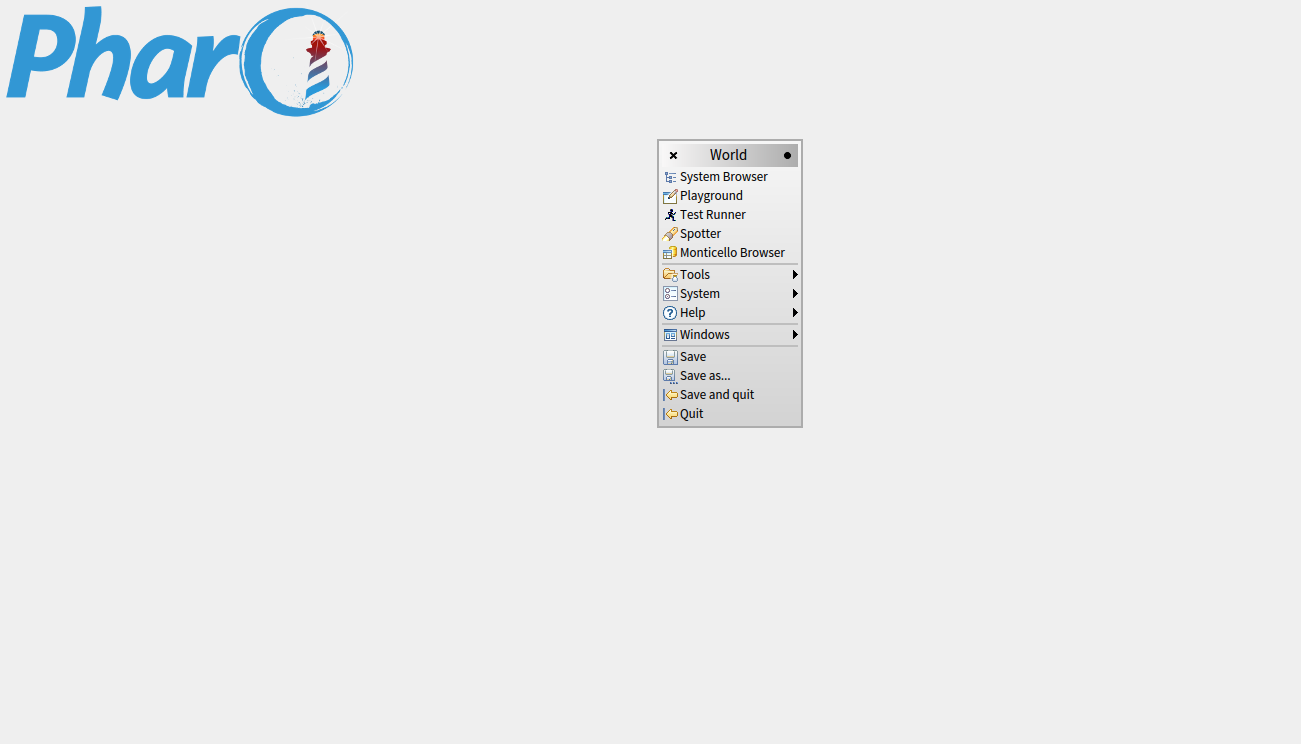
\includegraphics[width=1.0\textwidth]{figures/Pharo40.png}\caption{Pharo 4.0 window with World Menu activated.\label{worldMenu}}\end{center}
\end{figure}


Clicking anywhere on the background of the Pharo window will display the
World Menu. World Menu contains many of the Pharo tools, utilities and settings.

You will see a list of several core tools in Pharo, including the class browser
and the workspace.
\section{Install Kendrick}
From the the World Menu, select the \symbol{34}Tools\symbol{34} and after that the Configuration Browser.
Find in the Configuration Browser, the Kendrick configuration and select it. Click on \symbol{34}Install Stable version\symbol{34}.
You need to be connected to the Internet, in order to download the Kendrick package.
\section{Finding out the Examples package integrated in Kendrick}
From the World menu, select the \symbol{34}System Browser\symbol{34}.
Type \symbol{34}Kendrick\symbol{34} in the searching textbox to find the Kendrick packages then expanding \symbol{34}Kendrick\symbol{34}.
All the integrated examples of Kendrick could be found in the \symbol{34}Examples\symbol{34} package.
To run an example, from the World menu, select Workspace. In the Playground form, type a script to create an example and run it.
For example:
% syntax highlighting = smalltalk

\begin{code}{}
KEDeterministicExamples new exampleRK4SolverOnSIRSimpleModel
\end{code}

\textbf{KEDeterministicExamples}: class name.

\textbf{exampleRK4SolverOnSIRSimpleModel}: method name.

Then click on the play button to run the script. The result will be represented in the next view (Figure \ref{Playground})


\begin{figure}

\begin{center}
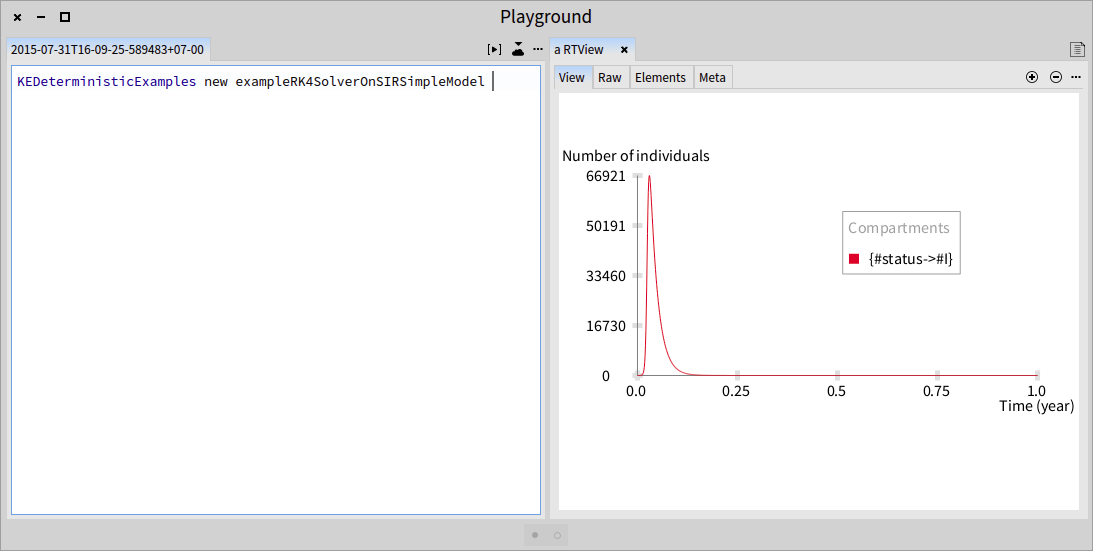
\includegraphics[width=1.0\textwidth]{figures/Playground.png}\caption{Run the script in the Playground.\label{Playground}}\end{center}
\end{figure}

\section{Launching models with simulation tools of Kendrick}
An epidemiological model can be interpreted to run a deterministic, stochastic or agent-based simulation.
The simulations are written once but for all the Kendrick models.

Once the model is specified, create new instance of KESimulator and determine the parameters of simulation such as: algorithm, starting time, ending time and the step.
For example:
% syntax highlighting = smalltalk

\begin{code}{}
simulator := KESimulator new: #RungeKutta from: 0.0 to: 1.0 step: 0.001.
simulator executeOn: model.
\end{code}

For this moment, the platform supported the algorithms: ODE Solvers (RungeKutta, Euler, etc.), Gillespie's direct, Explicit Tau Leap and Individual-based simulation.
The scripts following allows to create these simulations:
% syntax highlighting = smalltalk

\begin{code}{}
simulator := KESimulator new: #Gillespie from: 0.0 to: 1.0 step: 0.001.
simulator executeOn: model.
\end{code}


% syntax highlighting = smalltalk

\begin{code}{}
simulator := KESimulator new: #TauLeap from: 0.0 to: 1.0 step: 0.001.
simulator executeOn: model.
\end{code}


% syntax highlighting = smalltalk

\begin{code}{}
simulator := KESimulator new: #IBM from: 0.0 to: 1.0 step: 0.001.
simulator executeOn: model.
\end{code}


In Kendrick platform, the simulation results are stored as time series.
% syntax highlighting = smalltalk

\begin{code}{}
simulator allTimeSeries
\end{code}

This script will return an array of all time series.
To obtain the time series of a compartment, just indicate the name of this compartment as parameter of the function \symbol{34}timeSeriesAt\symbol{34}.
% syntax highlighting = smalltalk

\begin{code}{}
simulator timeSeriesAt: '{#status: #I}'
\end{code}

These scripts below allow to apply an additional function on the time series.
% syntax highlighting = smalltalk

\begin{code}{}
(simulator timeSeriesAt: '{#status: #I}') sqrt
\end{code}


% syntax highlighting = smalltalk

\begin{code}{}
(simulator timeSeriesAt: '{#status: #I}') log
\end{code}


The time series then are passed as data of the diagram builder to view the simulation results:
% syntax highlighting = smalltalk

\begin{code}{}
diag := (KEDiagramBuilder new) data: simulator allTimeSeries.
diag open
\end{code}

Other configurations of diagram:
% syntax highlighting = smalltalk

\begin{code}{}
diag xLabel: 'Time (years)'.
diag yLabel: 'Infectious'.
diag legendTitle: 'Vaccination rate'
\end{code}

By default, xLabel: Time (days), yLabel: Number of individuals, legendTitle: Compartments.
\chapter{Introduction to Simple Epidemic Model}
The targeted model of the \textbf{Kendrick} language is compartmental model such as the SIR, SEIR model ... in which the individuals are first considered as \textit{Susceptible} to pathogen (status S), then can be infected, assumed \textit{Infectious} (status I) that can spread the infection and \textit{Recovery} (status R) who are immunised and cannot become infected again. The transition of status between compartments is represented mathematically as derivatives of compartment size with respect to time.

At the moment, \textbf{Kendrick} supports for the mathematical models of epidemiology based on ordinary differential equations (\textbf{ODEs}). The system of ODEs followed represents the SIR classic model of epidemiology:


\begin{figure}

\begin{center}
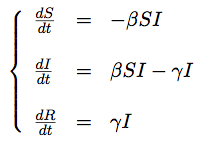
\includegraphics[width=0.35\textwidth]{figures/equation1.png}\caption{Mathematical description of SIR model using ODEs.\label{equation1}}\end{center}
\end{figure}


These models are specified using the Kendrick language and modeled using the simulation module integrated into the platform.
The simulator takes the Kendrick model (the epidemiological model written in Kendrick language) and performs a simulation algorithm and give out the result showing the spatial and temporal evolution dynamics of each compartment. This visualization is done by using Roassal.

The simulation module supports three modeling formalisms: deterministic, stochastic and individual-based (also called agent-based).
The modelers can switch between the simulation modes by indicating the algorithm used. At the moment, we use the RK4 method for deterministically resolving ODEs.
The stochastic simulation converts the ODEs of the model to events and using Gillespie's algorithms to generate stochastic model.
The individual-based simulator allows to reach the model at more detailed level.
\section{ Simple SIR (without births and deaths)}
Program 2.1 is a simple SIR model. These are the equations and the code of the model:
\subsection{ Equations}

\begin{equation}
\frac{dS}{dt} = -\beta*S*I
\end{equation}
\begin{equation}
\frac{dI}{dt} = \beta*S*I-\gamma*I
\end{equation}
\begin{equation}
\frac{dR}{dt} = \gamma*I
\end{equation}
\subsection{ Pharo code}
Here, we just demonstrate the code written in Smalltalk language to resolve the system of equations and view the results.
% syntax highlighting = smalltalk

\begin{code}{}
|solver system dt beta gamma values stepper diag colors maxTime st legend|
dt := 0.001.
beta := 0.0052.
gamma := 52.
maxTime := 1.
system := ExplicitSystem block: [ :x :t| |c|
     c := Array new: 3.
     c at: 1 put: (beta negated) * (x at: 1) * (x at: 2).
     c at: 2 put: (beta * (x at: 1) * (x at: 2)) - (gamma * (x at: 2)).
     c at: 3 put: gamma * (x at: 2).
     c
     ].
stepper := RungeKuttaStepper onSystem: system.
solver := (ExplicitSolver new) stepper: stepper; system: system; dt: dt.
st := { 99999. 1. 0}.
values := (0.0 to: maxTime by: dt) collect: [ :t| st := stepper doStep: st time: t stepSize: dt ].

diag := RTGrapher new.
diag extent: 400 @ 200.

colors := Array with: Color blue with: Color red with: Color green.
1 to: 3 do: [ :i|
	|ds|
	ds := RTDataSet new.
	ds points: (1.0 to: ((maxTime/dt)+1) by: 1).
	ds y: [ :x| (values at: x) at: i ].
	ds x: [ :t| (t - 1)*dt].
	ds noDot.
	ds connectColor: (colors at: i).
	diag add: ds ].
diag axisX title: 'Time (year)'.
diag axisY title: 'Number of individuals'.
diag axisY noDecimal.
legend := RTLegendBuilder new.
legend view: diag view.
legend addText: 'Compartments'.
legend addColor: (colors at: 1) text: '#status: #S'.
legend addColor: (colors at: 2) text: '#status: #I'.
legend addColor: (colors at: 3) text: '#status: #R'.
legend build.
diag build.
diag view @ RTZoomableView.
^ diag view
\end{code}

Executing this script we obtain the results of the system of equations as in Figure \ref{SIR_RK4_pharo}

\begin{figure}

\begin{center}
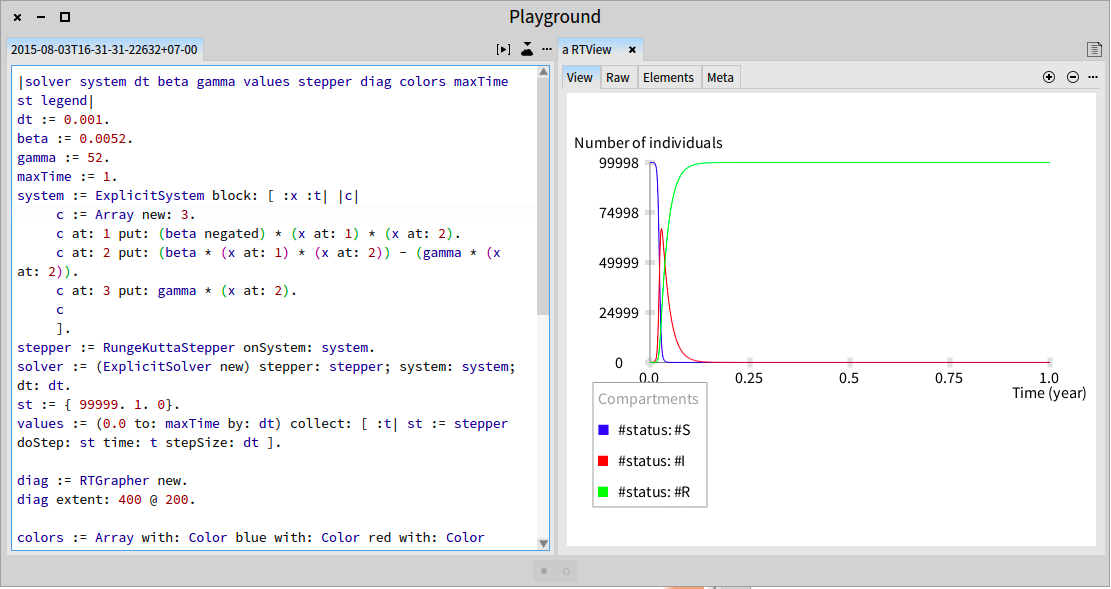
\includegraphics[width=1.0\textwidth]{figures/SIR_RK4_pharo.png}\caption{Deterministic dynamics of the SIR model using Smalltalk.\label{SIR_RK4_pharo}}\end{center}
\end{figure}

\subsection{ Kendrick code}
We use now the Kendrick DSL to express the SIR model.
We start to create an instance of KEModel and then enumerate the compartment names with their initial value.
In this model, we have 3 compartments S, I and R. The population has one attribute \textit{status}.
There is at least one infected in order to start the process.
Two transitions are added to the model, one from S to I and another one from I to R.
The parameters of the model  $\beta = 0.0052$ and $\gamma=52$.

% syntax highlighting = smalltalk

\begin{code}{}
| model |
	model := KEModel new.
  model population attributes: '{ #status: [#S, #I, #R] }'.
	model
		buildFromCompartments:
			'{
		{ #status: #S }: 99999,
		{ #status: #I }: 1,
		{ #status: #R }: 0
	}'.
	model addParameters: '{#beta: 0.0052, #gamma: 52}'.
	model
		addTransitionFrom: '{#status: #S}'
		to: '{#status: #I}'
		probability: [ :m | (m atParameter: #beta) * (m probabilityOfContact: '{#status:#I}') ].
	model addTransitionFrom: '{#status: #I}' to: '{#status: #R}' probability: [ :m | m atParameter: #gamma ].
\end{code}


Paste this script in the Workspace tool, define the simulations on this model, we obtain the results as in Figure \ref{SIR_RK4}.
We can find that, the two scripts returns identical results. As a DSL for epidemiology, using Kendrick is more simple.
Change the algorithm of simulation from \textit{RungeKutta} to \textit{Gillespie} and \textit{IBM} to investigate two other formalisms (stochastic and agent-based).
The results of these simulation are shown in Figure \ref{SIR_Gil} and Figure \ref{SIR_IBM}.


\begin{figure}

\begin{center}
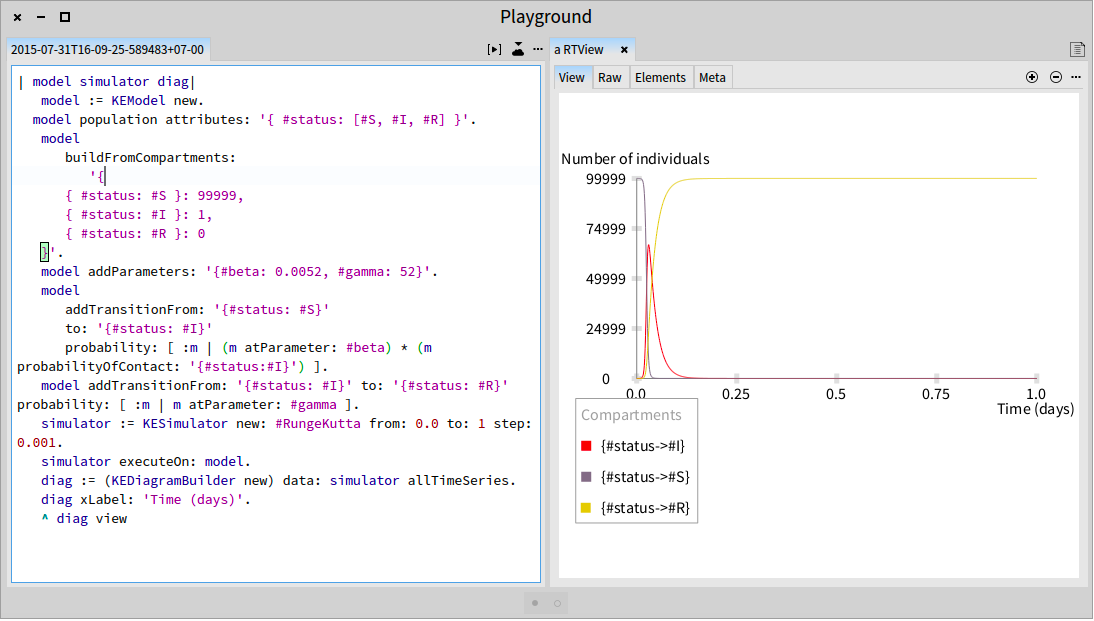
\includegraphics[width=1.0\textwidth]{figures/SIR_RK4.png}\caption{Deterministic dynamics of the SIR model without demography.\label{SIR_RK4}}\end{center}
\end{figure}



\begin{figure}

\begin{center}
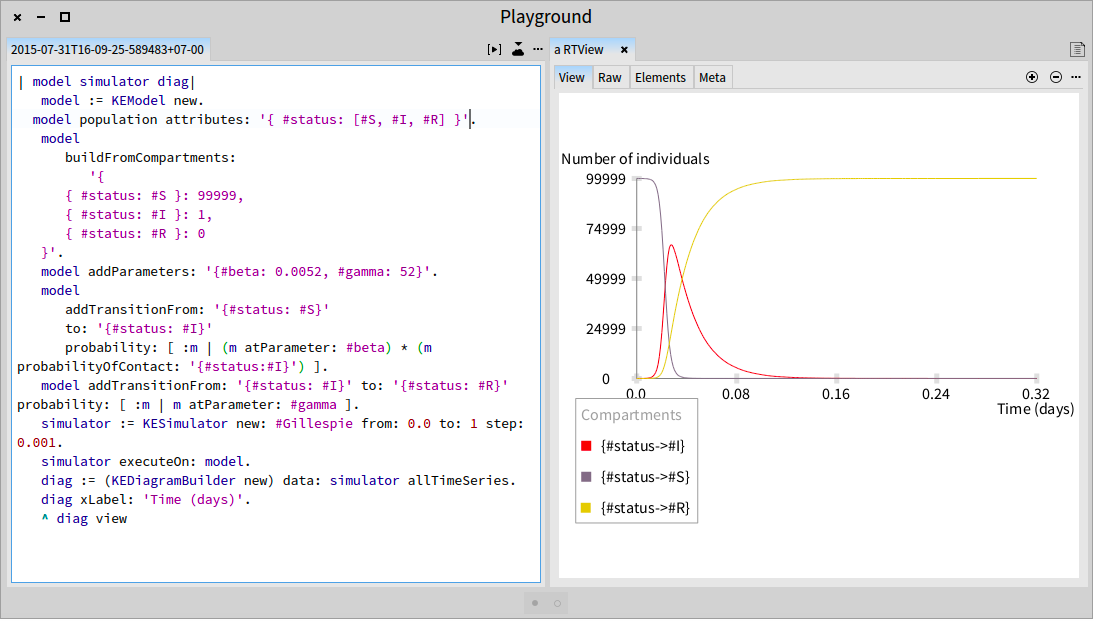
\includegraphics[width=1.0\textwidth]{figures/SIR_Gil.png}\caption{Using Gillespie's direct algorithm to study the dynamics of model.\label{SIR_Gil}}\end{center}
\end{figure}



\begin{figure}

\begin{center}
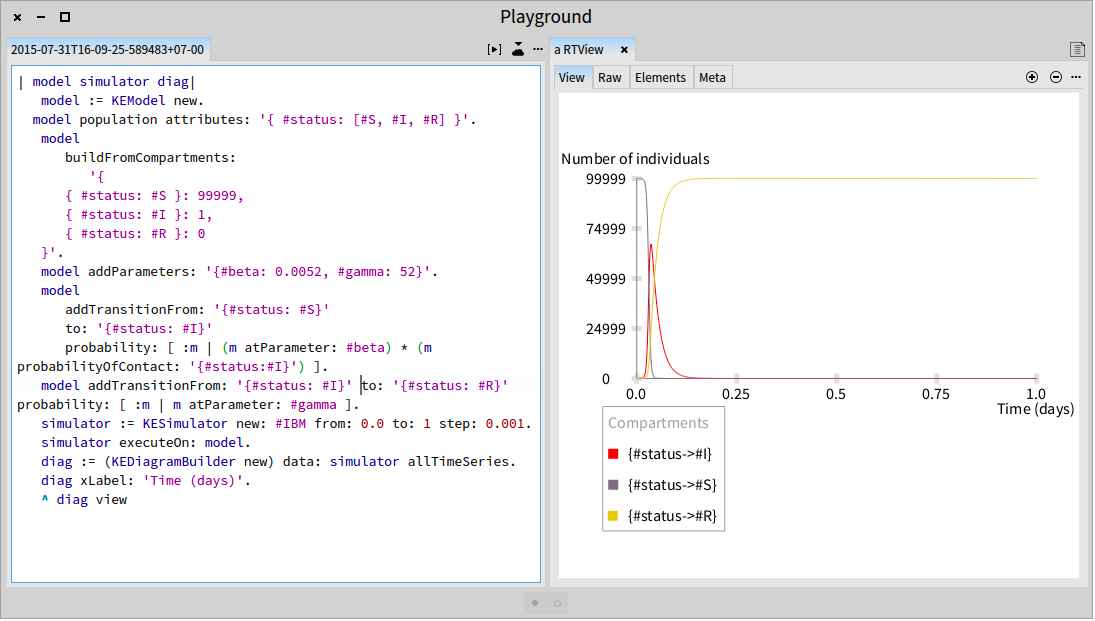
\includegraphics[width=1.0\textwidth]{figures/SIR_IBM.png}\caption{Agent-based approach to investigate the model at individual level.\label{SIR_IBM}}\end{center}
\end{figure}

\section{ SIR model with births and deaths}\subsection{ Equations}

\begin{equation}
\frac{dS}{dt} = \mu-\beta*S*I-\mu*S
\end{equation}
\begin{equation}
\frac{dI}{dt} = \beta*S*I-\gamma*I-\mu*I
\end{equation}
\begin{equation}
\frac{dR}{dt} = \gamma*I-\mu*R
\end{equation}
\subsection{ Pharo code}
% syntax highlighting = smalltalk

\begin{code}{}
|solver system dt beta gamma N values stepper diag mu colors maxTime st legend|
dt := 0.1.
mu := 5e-4.
beta := 1/5000.
gamma := 1/10.0.
N := 5000.
maxTime := 146.
system := ExplicitSystem block: [ :x :t| |c|
     c := Array new: 3.
     c at: 1 put: (mu*N) - (beta  * (x at: 1) * (x at: 2)) - (mu * (x at:1)).
     c at: 2 put: (beta * (x at: 1) * (x at: 2)) - (gamma * (x at: 2)) - (mu * (x at:2)).
     c at: 3 put: (gamma * (x at: 2)) - (mu * (x at: 3)).
     c
     ].

stepper := RungeKuttaStepper onSystem: system.
solver := (ExplicitSolver new) stepper: stepper; system: system; dt: dt.
st := #(4975 25 0).
values := (0.0 to: maxTime by: dt) collect: [ :t| st := stepper doStep: st
                                                          time: t stepSize: dt ].
diag := RTGrapher new.
diag extent: 400 @ 200.

colors := Array with: Color blue with: Color red with: Color green.
1 to: 3 do: [ :i|
	|ds|
	ds := RTDataSet new.
	ds points: (1.0 to: ((maxTime/dt)+1) by: 1).
	ds y: [ :x| (values at: x) at: i ].
	ds x: [ :t| (t - 1)*dt].
	ds noDot.
	ds connectColor: (colors at: i).
	diag add: ds ].
diag axisX title: 'Time (days)'.
diag axisY title: 'Number of individuals'.
diag axisY noDecimal.
legend := RTLegendBuilder new.
legend view: diag view.
legend addText: 'Compartments'.
legend addColor: (colors at: 1) text: '#status: #S'.
legend addColor: (colors at: 2) text: '#status: #I'.
legend addColor: (colors at: 3) text: '#status: #R'.
legend build.
diag build.
diag view @ RTZoomableView.
^ diag view
\end{code}

Running this script will give the results as can be seen in Figure \ref{SIR_Dem_RK4_pharo}


\begin{figure}

\begin{center}
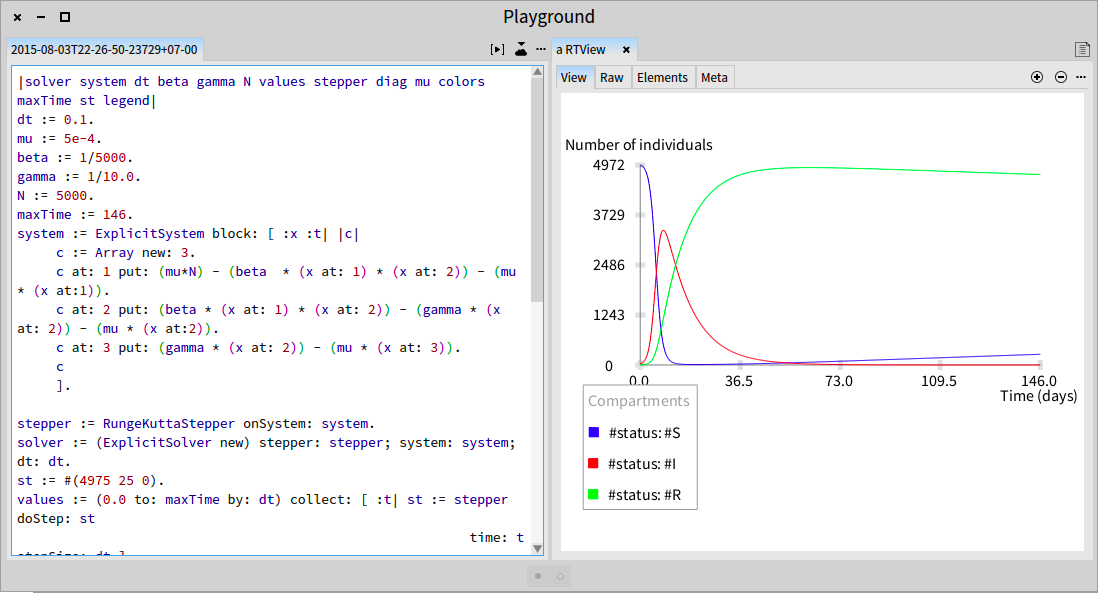
\includegraphics[width=1.0\textwidth]{figures/SIR_Dem_RK4_pharo.png}\caption{Resolving the system of equations of the SIR model with demography.\label{SIR_Dem_RK4_pharo}}\end{center}
\end{figure}

\subsection{Kendrick code}
Comparing to the previous model, in this model, it should add four other transitions. The first one represents the births of susceptible.
The three others represent the deaths of each compartment.
We use the ODE syntax to specify this model.

% syntax highlighting = smalltalk

\begin{code}{}
| model |
	model := KEModel new.
	model population attributes: '{#status: [#S, #I, #R]}'.
  model
		buildFromCompartments:
			'{
		{ #status: #S }: 4975,
		{ #status: #I }: 25,
		{ #status: #R }: 0
	}'.
	model addParameter: #beta value: 1 / 5000.
	model addParameter: #gamma value: 1 / 10.0.
	model addParameter: #mu value: 5e-4.
	model addParameter: #N value: #sizeOfPopulation.
	model addEquation: 'S:t=mu*N-beta*S*I-mu*S' parseAsAnEquation.
	model addEquation: 'I:t=beta*S*I-gamma*I-mu*I' parseAsAnEquation.
	model addEquation: 'R:t=gamma*I-mu*R' parseAsAnEquation.
\end{code}

Using deterministic simulation on this model we obtain the result as can be seen in Figure \ref{SIR_Dem_RK4}


\begin{figure}

\begin{center}
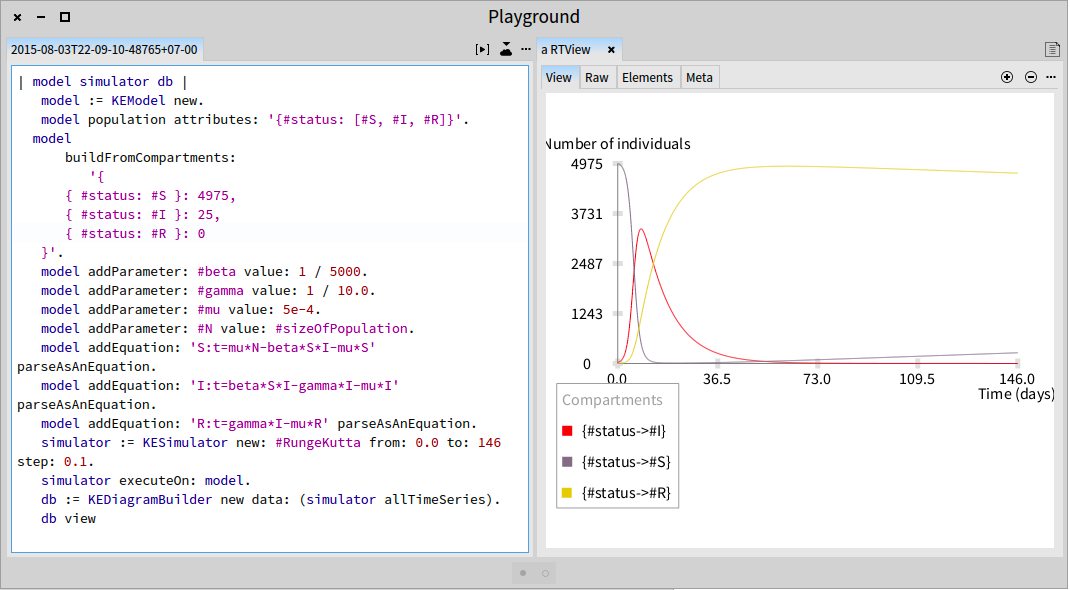
\includegraphics[width=1.0\textwidth]{figures/SIR_Dem_RK4.png}\caption{Deterministic dynamics of the SIR model with demography using Kendrick language.\label{SIR_Dem_RK4}}\end{center}
\end{figure}

\section{ SEIR model with births and deaths}
We introduce here a SEIR model. The E status means that a susceptible becomes infected but not yet infectious.
\subsection{Equations}

  \begin{equation}
    \frac{dS}{dt} = \mu*N - \beta*S*I - \mu*S
  \end{equation}
  \begin{equation}
    \frac{dE}{dt} = \beta*S*I - \sigma*E - \mu*E
  \end{equation}
  \begin{equation}
    \frac{dI}{dt} = \sigma*E - \gamma*I - \mu*I
  \end{equation}
  \begin{equation}
    \frac{dR}{dt} = \gamma*I - \mu*R
  \end{equation}
  
\subsection{Kendrick code}
Here, we use the parameters of measles model. The time unit is day.

% syntax highlighting = smalltalk

\begin{code}{}
  | model |
	model := KEModel new.
	model population attributes: '{#status: [#S, #E, #I, #R]}'.
	model
		buildFromCompartments:
			'{
		{#status: #S}: 99999,
		{#status: #I}: 1,
		{#status: #E}: 0,
		{#status: #R}: 0
	}'.
	model addParameters: '{
		#beta: 0.0000214,
		#gamma: 0.143,
		#mu: 0.0000351,
		#sigma: 0.125,
		#N: #sizeOfPopulation}'.
	model
		addTransitionFrom: '{#status: #S}'
		to: '{#status: #E}'
		probability: [ :m | (m atParameter: #beta) * (m probabilityOfContact: '{#status:#I}') ].
	model
		addTransitionFrom: '{#status: #E}'
		to: '{#status: #I}'
		probability: [ :m | m atParameter: #sigma ].
	model
		addTransitionFrom: '{#status: #I}'
		to: '{#status: #R}'
		probability: [ :m | m atParameter: #gamma ].
	model
		addTransitionFrom: '{#status: #S}'
		to: #empty
		probability: [ :m | m atParameter: #mu ].
	model
		addTransitionFrom: '{#status: #I}'
		to: #empty
		probability: [ :m | m atParameter: #mu ].
	model
		addTransitionFrom: '{#status: #R}'
		to: #empty
		probability: [ :m | m atParameter: #mu ].
	model
		addTransitionFrom: '{#status: #E}'
		to: #empty
		probability: [ :m | m atParameter: #mu ].
	model
		addTransitionFrom: #empty
		to: '{#status: #S}'
		probability: [ :m | m atParameter: #mu ].
\end{code}

\section{ SEIR model with vaccination at births}\subsection{ Equations}

  \begin{equation}
    \frac{dS}{dt} = \mu*N*(1-p) - \beta*S*I - \mu*S
  \end{equation}
  \begin{equation}
    \frac{dE}{dt} = \beta*S*I - \sigma*E - \mu*E
  \end{equation}
  \begin{equation}
    \frac{dI}{dt} = \sigma*E - \gamma*I - \mu*I
  \end{equation}
  \begin{equation}
    \frac{dR}{dt} = \mu*N*P + \gamma*I - \mu*R
  \end{equation}
  
\subsection{ Kendrick code}
% syntax highlighting = smalltalk

\begin{code}{}
| model |
	model := KEModel new.
	model population attributes: '{#status: [#S, #E, #I, #R]}'.
	model
		buildFromCompartments:
			'{
		{#status: #S}: 99999,
		{#status: #I}: 1,
		{#status: #E}: 0,
		{#status: #R}: 0
	}'.
	model addParameters: '{
		#beta: 0.00782,
		#gamma: 52.14,
		#mu: 0.0128,
		#sigma: 45.625,
		#N: #sizeOfPopulation,
		#p: 0.0}'.
	model
		addTransitionFrom: '{#status: #S}'
		to: '{#status: #E}'
		probability: [ :m | (m atParameter: #beta) * (m probabilityOfContact: '{#status:#I}') ].
	model
		addTransitionFrom: '{#status: #E}'
		to: '{#status: #I}'
		probability: [ :m | m atParameter: #sigma ].
	model
		addTransitionFrom: '{#status: #I}'
		to: '{#status: #R}'
		probability: [ :m | m atParameter: #gamma ].
	model
		addTransitionFrom: '{#status: #S}'
		to: #empty
		probability: [ :m | m atParameter: #mu ].
	model
		addTransitionFrom: '{#status: #I}'
		to: #empty
		probability: [ :m | m atParameter: #mu ].
	model
		addTransitionFrom: '{#status: #R}'
		to: #empty
		probability: [ :m | m atParameter: #mu ].
	model
		addTransitionFrom: '{#status: #E}'
		to: #empty
		probability: [ :m | m atParameter: #mu ].
	model
		addTransitionFrom: #empty
		to: '{#status: #S}'
		probability: [ :m | (m atParameter: #mu) * (1 - (m atParameter: #p)) ].
	model
		addTransitionFrom: #empty
		to: '{#status: #R}'
		probability: [ :m | (m atParameter: #mu) * (m atParameter: #p) ].
\end{code}

\section{ SEIR model with seasonal forcing}
The parameters of Kendrick model is not only a constant but also a temporal function as in this model.
\subsection{ Equations}

  \begin{equation}
    \frac{dS}{dt} = \mu*N - \beta_0*(1+\beta_{amp}*cos(t))*S*I - \mu*S
  \end{equation}
  \begin{equation}
    \frac{dE}{dt} = \beta_0*(1+\beta_{amp}*cos(t))*S*I - \sigma*E - \mu*E
  \end{equation}
  \begin{equation}
    \frac{dI}{dt} = \sigma*E - \gamma*I - \mu*I
  \end{equation}
  \begin{equation}
    \frac{dR}{dt} = \gamma*I - \mu*R
  \end{equation}
  
\subsection{ Kendrick code}
% syntax highlighting = smalltalk

\begin{code}{}
	| model |
	model := KEModel new.
	model population attributes: '{ #status: [#S, #E, #I, #R] }'.
	model
		buildFromCompartments:
			'{
		{ #status: #S }: 99999,
		{ #status: #E }: 0,
		{ #status: #I }: 1,
		{ #status: #R }: 0
	}'.
	model addParameters: '{
		#beta0: 0.0052,
		#gamma: 52,
		#sigma: 52,
		#betaAmp: 0.3,
		#N: #sizeOfPopulation,
		#mu: 0.0125}'.
	model
		addParameter: #beta
		value: 'beta0*(1 + (betaAmp*cos(t)))' parseAsAnExpression.
	model
		addEquation: 'S:t=mu*N-beta*S*I-mu*S' parseAsAnEquation.
	model
		addEquation: 'E:t=beta*S*I-sigma*E-mu*E' parseAsAnEquation.
	model
		addEquation: 'I:t=sigma*E-gamma*I-mu*I' parseAsAnEquation.
	model
		addEquation: 'R:t=gamma*I-mu*R' parseAsAnEquation.
\end{code}

\chapter{ Heterogeneous Host Models}\section{ SIS model with multiple risk groups}
We consider here the the SIS model in which the population is structured into multiple risk groups (host-heterogeneous model) labelled 1, 2, ...
The group labelled 1 is the lowest risk. The group labelled 5 is the highest risk.
\subsection{ Equations}

  \begin{equation}
    \frac{dS_i}{dt} = \gamma_i I_i - \sum_j \beta_{ij} S_i I_j
  \end{equation}
  \begin{equation}
    \frac{dI_i}{dt} = \sum_j \beta_{ij} S_i I_j - \gamma_i I_i
  \end{equation}
  
\subsection{ Kendrick model}
% syntax highlighting = smalltalk

\begin{code}{}
| model graph |
	model := KEModel new.
	model population: KEMetaPopulation new.
	model population attributes: {#riskGroup->(1 to: 5). #status->#(S I)}.
	model
		buildFromAttributes: #(#status #riskGroup)
		compartments: {
		  (#(#S 1) -> 6000). (#(#I 1) -> 0).
        (#(#S 2) -> 31000). (#(#I 2) -> 0).
        (#(#S 3) -> 52000). (#(#I 3) -> 0).
        (#(#S 4) -> 8000). (#(#I 4) -> 0).
        (#(#S 5) -> 2999). (#(#I 5) -> 1).
		}.
	model addParameter: #beta value: 16e-9.
	model addParameter: #gamma value: 0.2.

	graph := KEContactNetwork
					newOn: model population
					atAttribute: #riskGroup.
	graph edges: { 2->2. 2->3. 2->4. 2->5. 3->3. 3->4. 3->5. 4->4. 4->5. 5->5 };
			strengthOfConnections: #(9 30 180 300 100 600 1000 3600 6000 10000).

	model addEquation: 'S:t=gamma*I-beta*S*I' parseAsAnEquation.
	model addEquation: 'I:t=beta*S*I-gamma*I' parseAsAnEquation.
\end{code}

\chapter{ Multi-Pathogen$/$Multi-Host Models}\section{ SIR model with three species of hosts}
In the standard models of epidemiology, the population is compartmentalized by only clinic status.
As such, the population has only one degree of subdivision.
In a context of multi-host (multi-species) model, the host population has two degrees of subdivision due to the attribute species of each individual.
\subsection{ Equations}

  \begin{equation}
    \frac{dS}{dt} = \mu_i*N_i - \sum_j \beta_{ij}*S_i*I_j - \mu_i*S_i
  \end{equation}
  \begin{equation}
    \frac{dI}{dt} = \sum_j \beta_{ij}*S_i*I_j - \gamma_i*I_i - \mu_i*I_i
  \end{equation}
  \begin{equation}
    \frac{dR}{dt} = \gamma_i*I_i - \mu_i*R_i
  \end{equation}
  
\subsection{ Configurations of Kendrick model}
In epidemiology, it is important to distinguish between two basic assumptions in terms of the underlying structure of contacts within the population.
Either the model is assumed to be mass action or pseudo mass action.
The first kind reflects the situation where the number of contacts is independent of the population size.
So that the force of infection  $\lambda = \beta I / N$.
In some circumstances, the transmission rate  $\beta$ is rescaled by  $N$.
The second one assumes that as the population size increases, so does the contact rate.
As such the force of infection  $\lambda = \beta I$.

At the moment, Kendrick model includes three parameters of configuration: sizeOfPopulation, rescale, mass\_action.
By default:

% syntax highlighting = smalltalk

\begin{code}{}
#sizeOfPopulation->#population
#rescale->true
#mass_action->true
\end{code}


In the context of the multi-species model, it is important to config the size of population for each species.
As such:

% syntax highlighting = smalltalk

\begin{code}{}
model configurations: {#sizeOfPopulation->#(#species)}
\end{code}

\subsection{ Kendrick model}
In this model, we define the parameter  $\mu$ for three scopes corresponding to each species.
In order to represent the interaction between three species, we define a contact network.
Due to this network, the force of infection will be modified as:

  \begin{equation}
    \lambda = \beta * \sum_j \rho_{ij} * I_j
  \end{equation}
  
where  $\rho_{ij}$ denotes the strength of connection between species  $i$ and  $j$.

% syntax highlighting = smalltalk

\begin{code}{}
| model graph |
	model := KEModel new.
	model
		population:
			(KEMetaPopulation new
				attributes:
					{(#status -> #(#S #I #R)).
					(#species -> #(#mosquito #reservoir1 #reservoir2))}).
	model
		buildFromAttributes: #(#status #species)
		compartments:
			{(#(#S #mosquito) -> 9800).
			(#(#I #mosquito) -> 200).
			(#(#R #mosquito) -> 0).
			(#(#S #reservoir1) -> 1000).
			(#(#I #reservoir1) -> 0).
			(#(#R #reservoir1) -> 0).
			(#(#S #reservoir2) -> 2000).
			(#(#I #reservoir2) -> 0).
			(#(#R #reservoir2) -> 0)}.
	model addParameter: #mu
		   inScopes: {
				#species->#mosquito.
				#species->#reservoir1.
				#species->#reservoir2}
		   values: #(12.17 0.05 0.05).
	model addParameter: #gamma value: 52.
	model addParameter: #beta value: 1.
	model addParameter: #N value: #sizeOfPopulation.
	model configurations: { #sizeOfPopulation->#(#species) }.

	graph := KEContactNetwork
			newOn: model population
			atAttribute: #species.
	graph edges: { #mosquito->#reservoir1. #mosquito->#reservoir2 };
			strengthOfAllConnections: 0.02.
	model
		addTransitionFrom: '{#status: #S}'
		to: '{#status: #I}'
		probability: [ :m | (m atParameter: #beta) * (m probabilityOfContact: '{#status: #I}') ].
	model
		addTransitionFrom: '{#status: #I}'
		to: '{#status: #R}'
		probability: [ :m | m atParameter: #gamma ].
	model
		addTransitionFrom: '{#status: #S}'
		to: #empty
		probability: [ :m | m atParameter: #mu ].
	model
		addTransitionFrom: '{#status: #I}'
		to: #empty
		probability: [ :m | m atParameter: #mu ].
	model
		addTransitionFrom: '{#status: #R}'
		to: #empty
		probability: [ :m | m atParameter: #mu ].
	model
		addTransitionFrom: #empty
		to: '{#status: #S}'
		probability: [ :m | m atParameter: #mu ].
\end{code}

\chapter{ Spatial models}\section{ SEIR model with spatial dynamics}
We investigate the impact of spatial effects.
Considering a spatial model organised by n patches arranged in a ring.
The individuals can move between two neighbouring patches.
In each patch, we have a sub-population with four compartments S, E, I and R.
To specify this model, we use the Migration Network built in Kendrick. Due to this network, the model will have migration transitions from one compartment to other.
\subsection{ Equations}

  \begin{equation}
    \frac{dS_i}{dt} = \mu_i N_i - \beta_i S_i I_i - \mu_i S_i - \sum_j \rho_{ij} S_i + \sum_j \rho_{ji} S_j
  \end{equation}
  \begin{equation}
    \frac{dE_i}{dt} = \beta_i S_i I_i - \mu E_i - \varepsilon E_i - \sum_j \rho_{ij} E_i + \sum_j \rho_{ji} E_j
  \end{equation}
  \begin{equation}
    \frac{dI_i}{dt} = \varepsilon E_i - \mu I_i - \gamma_i I_i - \sum_j \rho_{ij} I_i + \sum_j \rho_{ji} I_j
  \end{equation}
  \begin{equation}
    \frac{dR_i}{dt} = \gamma_i I_i - \mu R_i - \sum_j \rho_{ij} R_i + \sum_j \rho_{ji} R_j
  \end{equation}
  
\subsection{ Kendrick model}
% syntax highlighting = smalltalk

\begin{code}{}
| model graph |
model := KEModel new.
model population: KEMetaPopulation new.
model population attributes: {
	#patch->((1 to: 5)).
	#status->#(S E I R)}.
model
	buildFromAttributes: #(#status #patch)
	compartments: {
		  (#(#S 1) -> 900). (#(#E 1) -> 0). (#(#I 1) -> 100). (#(#R 1) -> 0).
        (#(#S 2) -> 1000). (#(#E 2) -> 0). (#(#I 2) -> 0). (#(#R 2) -> 0).
        (#(#S 3) -> 1000). (#(#E 3) -> 0). (#(#I 3) -> 0). (#(#R 3) -> 0).
        (#(#S 4) -> 1000). (#(#E 4) -> 0). (#(#I 4) -> 0). (#(#R 4) -> 0).
        (#(#S 5) -> 1000). (#(#E 5) -> 0). (#(#I 5) -> 0). (#(#R 5) -> 0).
	}.
model
	addParameter: #beta
	inScopes: {
		(#patch->1).
		(#patch->2).
		(#patch->3).
		(#patch->4).
		(#patch->5)
	}
	values: #(0.75 0.5 0.5 0.5 0.5).
model addParameter: '{
	#v: 0.00274,
	#d: 0.0000365,
	#epsilon: 0.5,
	#gamma: 0.25,
	#N: #sizeOfPopulation}'.
model configurations: {
		#sizeOfPopulation->#(#patch).
		#rescale->false }.
graph := KEMigrationNetwork
				newOn: model population
				atAttribute: #patch
				topology: (KERandomSmallWorldNetwork new K: 2; beta: 0).
graph strengthOfAllConnections: 0.03.
graph addMigrationTransitionsTo: model.

model addEquation: 'S:t=d*N-d*S-beta*S*I+v*R' parseAsAnEquation.
model addEquation: 'E:t=beta*S*I-d*E-epsilon*E' parseAsAnEquation.
model addEquation: 'I:t=epsilon*E-d*I-gamma*I' parseAsAnEquation.
model addEquation: 'R:t=gamma*I-d*R-v*R' parseAsAnEquation.
\end{code}



% another try
% \printglossary
\bibliographystyle{jurabib}
\bibliography{scg}

\printindex

\end{document}

%=================================================================
%%% Local Variables:
%%% coding: utf-8
%%% mode: latex
%%% TeX-master: t
%%% TeX-PDF-mode: t
%%% ispell-local-dictionary: "english"
%%% End:
